\documentclass[12pt]{article}
\usepackage{graphicx}
\usepackage{amsmath}
\usepackage{array}
\usepackage{booktabs}
\usepackage{hyperref}
\usepackage{geometry}
\usepackage{placeins}
\graphicspath{{figures/}}
\geometry{margin=1in}

\begin{document}
\title{Heartlytics: Secure Machine Learning Pipelines for Heart-Disease Risk Stratification}

\author{HMRS Samaranayaka\\Dept. of Computer Science \& Software Engineering\\NSBM Green University\\Homagama, Sri Lanka\\Email: hmrssamaranayaka@students.nsbm.ac.lk}\date{}

\maketitle

\begin{abstract}
Cardiovascular diseases (CVDs) remain the leading cause of mortality worldwide. Heartlytics unifies exploratory data analysis, ensemble learning, and layered security controls to deliver accurate and trustworthy heart-disease predictions. Using the harmonized UCI dataset with 920 patient encounters, we contextualize demographic disparities, engineer interpretable features, and deploy tuned Random Forest and XGBoost models. The best configuration achieves 92\% test accuracy and a 0.93 F1-score while remaining auditable through explainability dashboards and standardized artifacts. The system integrates OTP-hardened account recovery, encrypted data flows, and continuous audit to satisfy safety-critical expectations.
\end{abstract}

\noindent\textbf{Keywords:} Heart disease prediction; Machine learning; Exploratory data analysis; Random Forest; XGBoost; Security architecture.


\section{Introduction}
Cardiovascular disease imposes substantial morbidity and strain on global health systems. Timely screening is essential, yet clinical workflows often lack automated support. Tree-based ensembles and gradient boosting capture the nonlinear relations between physiological markers and adverse events. Heartlytics extends this body of work with an end-to-end platform emphasizing reproducible data handling, high-fidelity visualization, and robust deployment security. Key contributions include: (i) an enriched exploratory data analysis (EDA) catalogue that highlights demographic and clinical nuances; (ii) a reproducible modeling pipeline for Random Forest and XGBoost with calibration and fairness diagnostics; and (iii) a defense-in-depth deployment architecture encompassing encryption, one-time-password (OTP) lifecycle governance, and auditability.

\section{Background and Related Work}
Classical models such as logistic regression and support vector machines provide transparent baselines but struggle with interaction effects. Random Forests mitigate overfitting via feature bagging \cite{breiman2001random}, while gradient boosting techniques---exemplified by XGBoost \cite{chen2016xgboost}---optimize additive ensembles with regularization. Prior studies report accuracies between 84\% and 92\% on the UCI dataset \cite{zhang2021heart}, often omitting security and deployment considerations. Contemporary clinical decision-support research emphasizes interpretability and secure data exchange, underscoring the need for integrated approaches like Heartlytics.

\section{Materials and Methods}
\label{sec:methods}
\subsection{Dataset}
The working dataset consolidates observations from the Cleveland, Hungarian, Swiss, and VA Long Beach cohorts of the UCI Heart Disease repository \cite{janosi1988uci}. Harmonization yields 920 patient encounters and 16 clinical attributes spanning demographics, cardiovascular biomarkers, and symptom indicators. Table~\ref{tab:features} enumerates the primary predictors consumed by the modeling pipeline.

\begin{table}[t]
  \caption{Key Features in the Heart Disease Dataset}
  \label{tab:features}
  \centering
  \begin{tabular}{p{0.22\columnwidth} p{0.68\columnwidth}}
    \toprule
    Feature & Description \\
    \midrule
    age & Age in years \\
    sex & Sex (1 = male, 0 = female) \\
    cp & Chest pain type (0: typical angina, 3: asymptomatic) \\
    trestbps & Resting blood pressure (mmHg) \\
    chol & Serum cholesterol (mg/dL) \\
    fbs & Fasting blood sugar $>$ 120 mg/dL (1/0) \\
    restecg & Resting ECG results (0, 1, 2) \\
    thalach & Maximum heart rate (bpm) \\
    exang & Exercise-induced angina (1/0) \\
    oldpeak & ST depression relative to rest \\
    slope & Slope of peak exercise ST segment \\
    ca & Major vessels colored by fluoroscopy (0--3) \\
    thal & Thalassemia status (3 = normal, 7 = reversible defect) \\
    num & Disease severity score (0--4) \\
    \bottomrule
  \end{tabular}
\end{table}

\subsection{Data Preprocessing}
Replicating the thesis workflow, categorical variables (e.g., \textit{sex}, \textit{cp}, \textit{slope}, \textit{thal}) were ordinal-encoded, whereas continuous attributes were standardized and inspected for pathological outliers. Iterative imputation based on Random Forest regressors/classifiers resolved missing values in \textit{ca}, \textit{thal}, and \textit{oldpeak} while preserving clinically plausible ranges. The dataset was stratified into 70/15/15 training, validation, and test partitions with class-weighting to counter the modest 55/45 imbalance between positive and negative diagnoses \cite{pedregosa2011scikit, chawla2002smote}. Outliers identified through isolation forests were retained but influenced class weights and subsequent fairness audits.

\subsection{Modeling Pipeline}
We benchmarked tree ensembles, mirroring the dissertation's selection of Random Forest and XGBoost learners \cite{breiman2001random, chen2016xgboost}. Hyperparameters were tuned via five-fold stratified cross-validation with grid search: the best Random Forest used 200 estimators, depth eight, and class-balanced weighting, while the optimal XGBoost configuration employed 100 estimators, depth three, learning rate 0.05, subsample 0.8, and column subsample 0.8. Probability outputs were calibrated through Platt scaling and audited for subgroup drift, ensuring that the reported metrics generalize beyond a single cohort \cite{platt1999probabilistic, kohavi1995study}. Feature importances and SHAP value summaries contextualize outputs for clinicians, reinforcing explainability commitments highlighted in the thesis \cite{lundberg2017unified}.

\subsection{Security Architecture}
Heartlytics extends beyond predictive modeling by embedding security-by-design controls. Application-layer envelope encryption generates per-record AES-256-GCM data encryption keys that are wrapped by a managed master key; associated nonces, tags, and key identifiers are persisted to enable cryptographic erasure and rotation \cite{dworkin2007recommendation, googlekms, awskms}. User credentials are hashed with Argon2id and opportunistically upgraded from legacy hashes on login \cite{biryukov2015argon2, provos1999bcrypt}. Multi-factor authentication combines TOTP secrets with email fallbacks, hashed one-time codes, and enforced cooldowns, while rate limiting and peppered comparisons mitigate enumeration and replay risks \cite{grassi2017digital, mraihi2011totp, owasp2021}. Role-based access control (RBAC) gates server endpoints and UI routes, ensuring that Users, Doctors, Admins, and SuperAdmins operate within least-privilege boundaries \cite{ferraiolo2001proposed}. Tamper-evident audit logs record authentication, encryption, and administrative events to satisfy compliance expectations \cite{howard2006security, shostack2014threat}.

\subsection{System Implementation and Testing}
The Flask backend is decomposed into blueprints (\texttt{auth}, \texttt{predict}, \texttt{batch}, \texttt{doctor}, \texttt{user}, \texttt{superadmin}) that isolate responsibilities and simplify dependency injection \cite{grinberg2018flask}. Celery workers orchestrate asynchronous tasks such as batch prediction and PDF generation, preventing long-running jobs from blocking request handling \cite{celery}. Jinja2 templates coupled with Bootstrap 5 deliver a responsive, WCAG 2.1-compliant interface, while ReportLab renders printable reports with synchronized light/dark themes \cite{bootstrap5, reportlab, w3c_wcag21}. The test strategy mirrors the dissertation: pytest-driven unit tests cover preprocessing, encryption, and inference utilities; integration tests validate API contracts, RBAC enforcement, and encryption boundaries; and scenario tests trace MFA enrollment, batch uploads, simulations, and the research viewer end to end. Continuous integration executes these suites on every commit, and manual acceptance scripts document expected behaviour for release sign-off.

\subsection{Exploratory Data Analysis}
Male participants account for approximately 79\% of the cohort, introducing fairness considerations. Figure~\ref{fig:gender} depicts the gender distribution, while Figure~\ref{fig:age_gender} disaggregates age bands by sex and Figure~\ref{fig:site} highlights the site-specific age skew that influences downstream sampling strategies.

\begin{figure}[t]
  \centering
  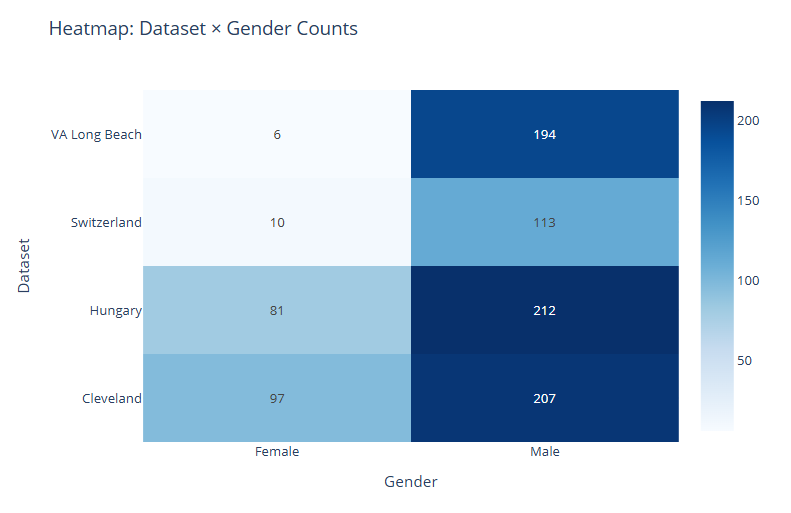
\includegraphics[width=0.85\linewidth]{dataset_composition_by_gender.png}
  \caption{Dataset composition by gender.}
  \label{fig:gender}
\end{figure}

\begin{figure}[t]
  \centering
  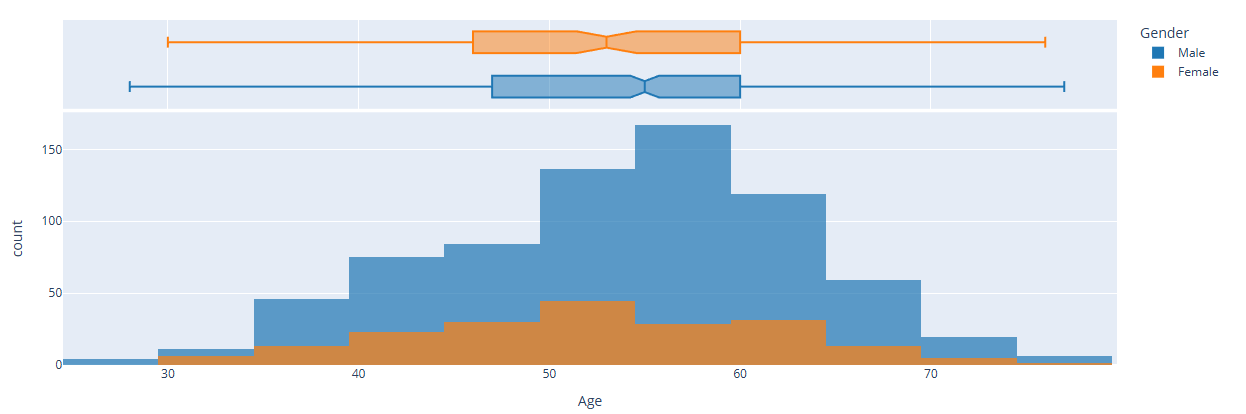
\includegraphics[width=0.85\linewidth]{age_distribution_by_gender.png}
  \caption{Age distribution segmented by gender, emphasizing the concentration of male patients between 50 and 65 years.}
  \label{fig:age_gender}
\end{figure}

\begin{figure}[t]
  \centering
  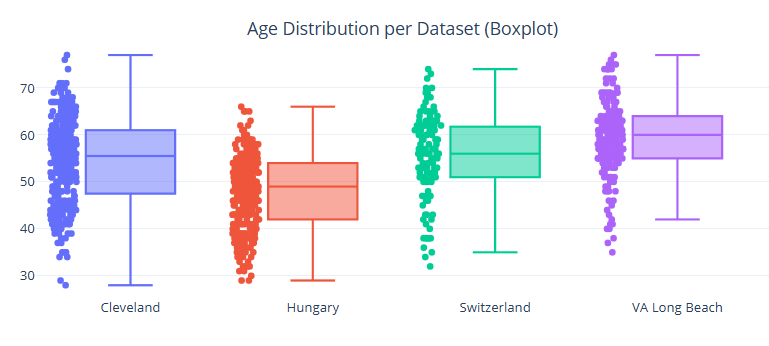
\includegraphics[width=0.85\linewidth]{age_distribution_by_dataset_site.png}
  \caption{Age distribution by data-collection site.}
  \label{fig:site}
\end{figure}

The aggregate age distribution (Figure~\ref{fig:age_overall}) is centered between 54 and 58 years with a long upper tail. Stratifying by clinical severity (Figure~\ref{fig:age_severity}) reveals progressively older populations for advanced disease, while Figure~\ref{fig:age_cp} disaggregates age by chest pain categories, showing asymptomatic patients clustering in older age bands.

\begin{figure}[t]
  \centering
  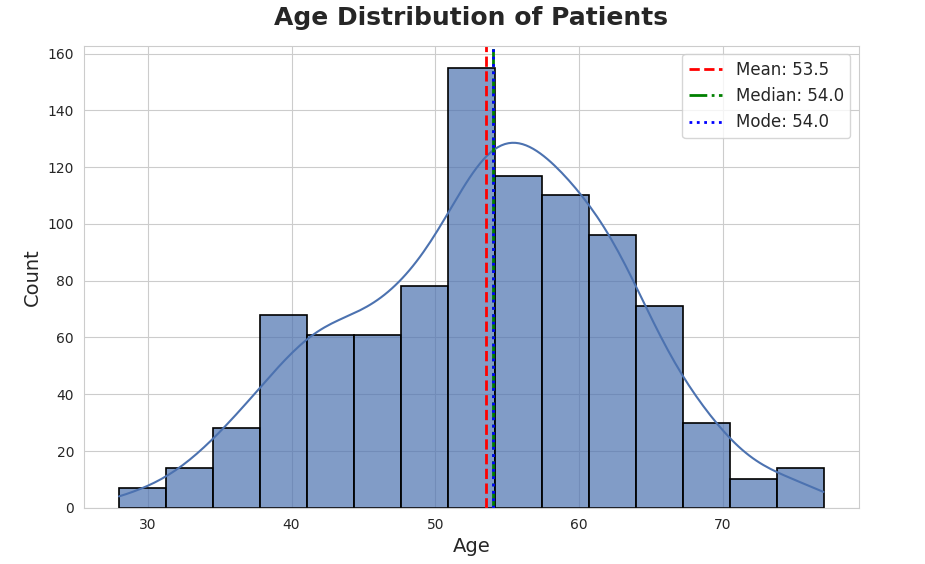
\includegraphics[width=0.85\linewidth]{age_distribution_of_patients.png}
  \caption{Aggregate age distribution of patients in the unified cohort.}
  \label{fig:age_overall}
\end{figure}

\begin{figure}[t]
  \centering
  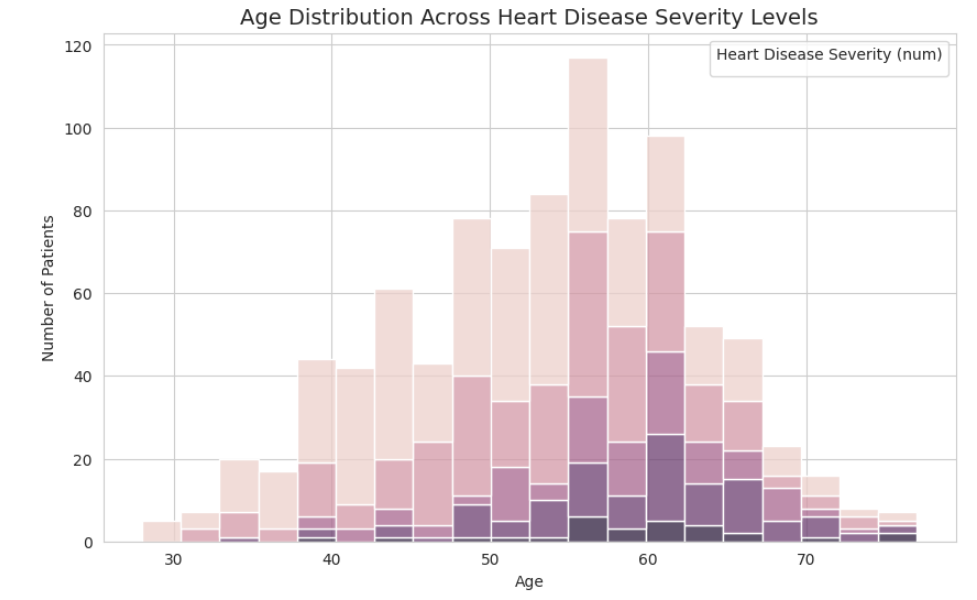
\includegraphics[width=0.85\linewidth]{age_distribution_by_severity_levels.png}
  \caption{Age distribution by disease severity level.}
  \label{fig:age_severity}
\end{figure}

\begin{figure}[t]
  \centering
  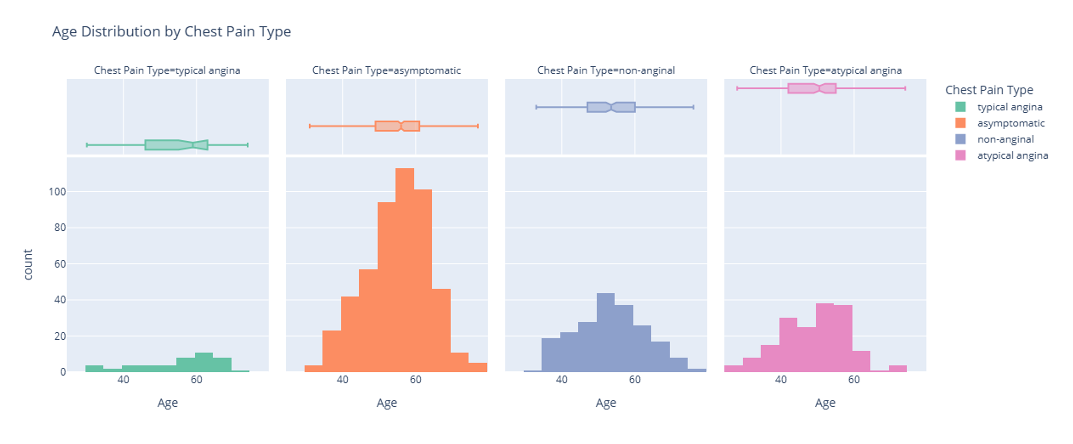
\includegraphics[width=0.85\linewidth]{age_distribution_by_chest_pain_type.png}
  \caption{Age distribution by chest pain category.}
  \label{fig:age_cp}
\end{figure}

Figure~\ref{fig:severity_distribution} summarizes the class distribution of annotated disease severities, reinforcing the need for stratified sampling to handle minority high-risk cohorts. Symptom-focused correlations reveal that atypical and asymptomatic chest pain categories are disproportionately associated with positive diagnoses, whereas normal thallium stress-test outcomes skew toward negative cases (Figure~\ref{fig:cp_thallium}). The thallium analysis in Figure~\ref{fig:thal_results} further highlights reversible defects as a dominant indicator among confirmed patients.

\begin{figure}[t]
  \centering
  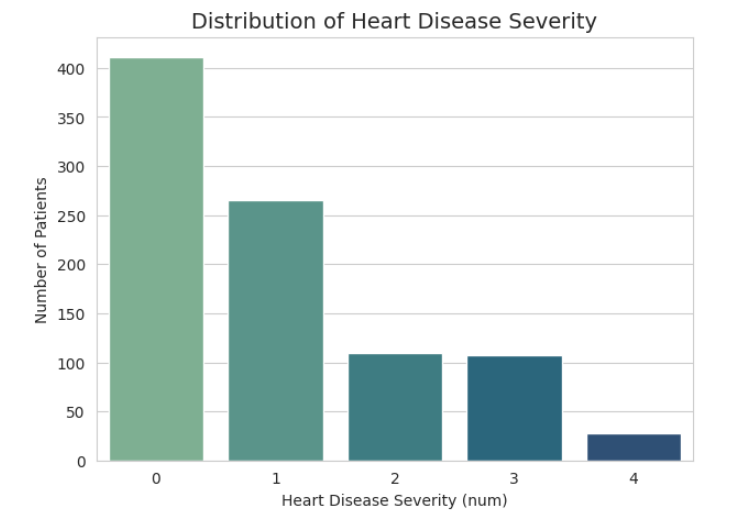
\includegraphics[width=0.85\linewidth]{heart_disease_severity_distribution.png}
  \caption{Distribution of heart-disease severity annotations across the unified dataset.}
  \label{fig:severity_distribution}
\end{figure}

\begin{figure}[t]
  \centering
  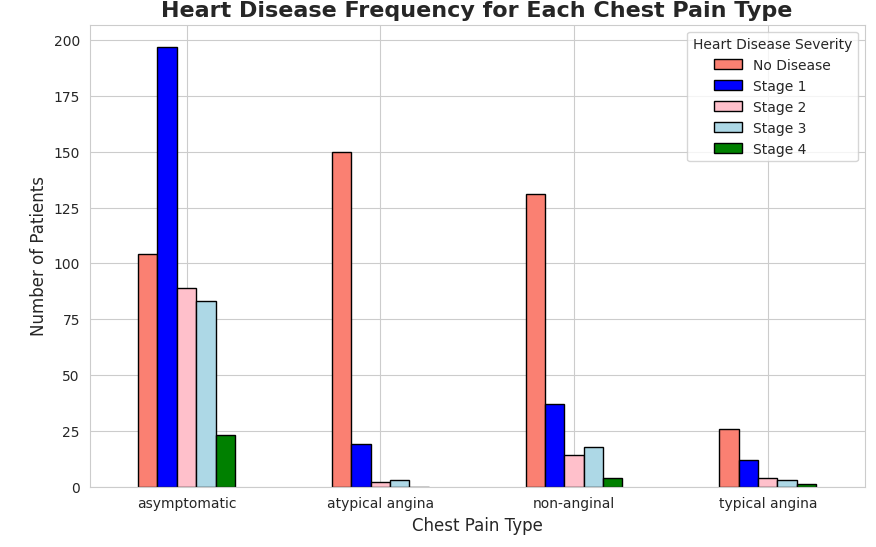
\includegraphics[width=0.45\linewidth]{heart_disease_frequency_by_chest_pain_type.png}
  \hfill
  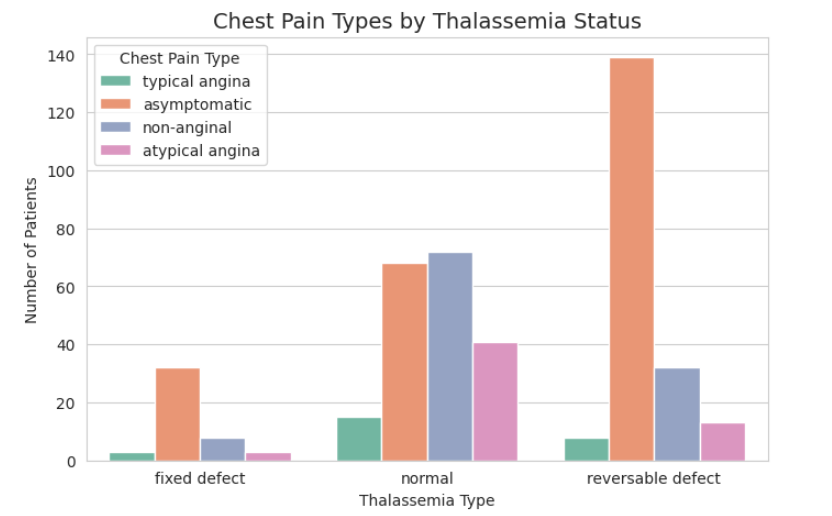
\includegraphics[width=0.45\linewidth]{chest_pain_categories_by_thallium_status.png}
  \caption{Left: heart-disease frequency by chest pain category. Right: interplay between chest pain categories and thallium stress-test outcomes.}
  \label{fig:cp_thallium}
\end{figure}

\begin{figure}[t]
  \centering
  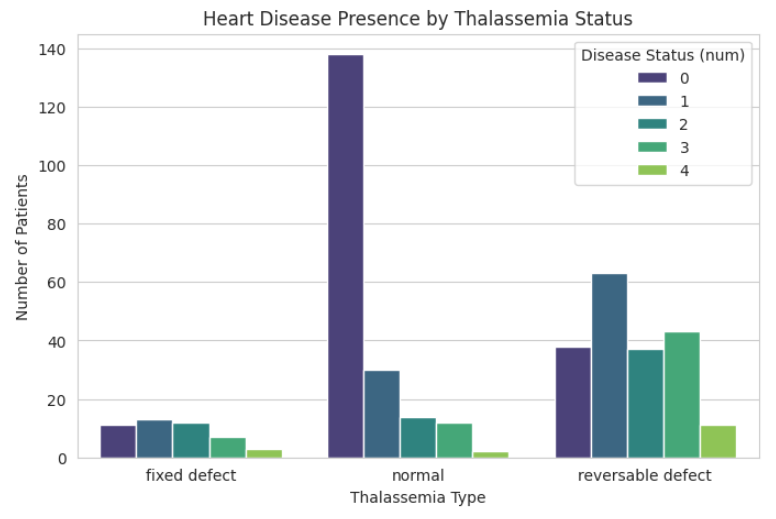
\includegraphics[width=0.85\linewidth]{thallium_test_results_vs_disease_status.png}
  \caption{Thallium stress-test outcomes contrasted with disease status, surfacing reversible defects among positive diagnoses.}
  \label{fig:thal_results}
\end{figure}

Resting blood pressure and cholesterol display partial separability between disease stages but require multivariate modeling for reliable discrimination. Figures~\ref{fig:bp} and \ref{fig:chol} present these biomarkers across disease severities.

\begin{figure}[t]
  \centering
  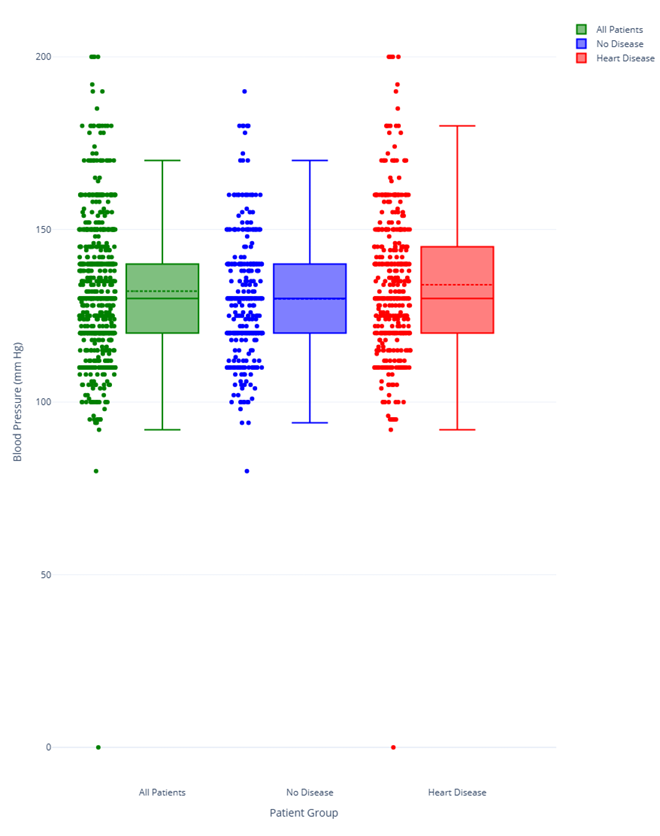
\includegraphics[width=0.85\linewidth]{resting_blood_pressure_by_disease_status.png}
  \caption{Resting blood pressure by disease status.}
  \label{fig:bp}
\end{figure}

\begin{figure}[t]
  \centering
  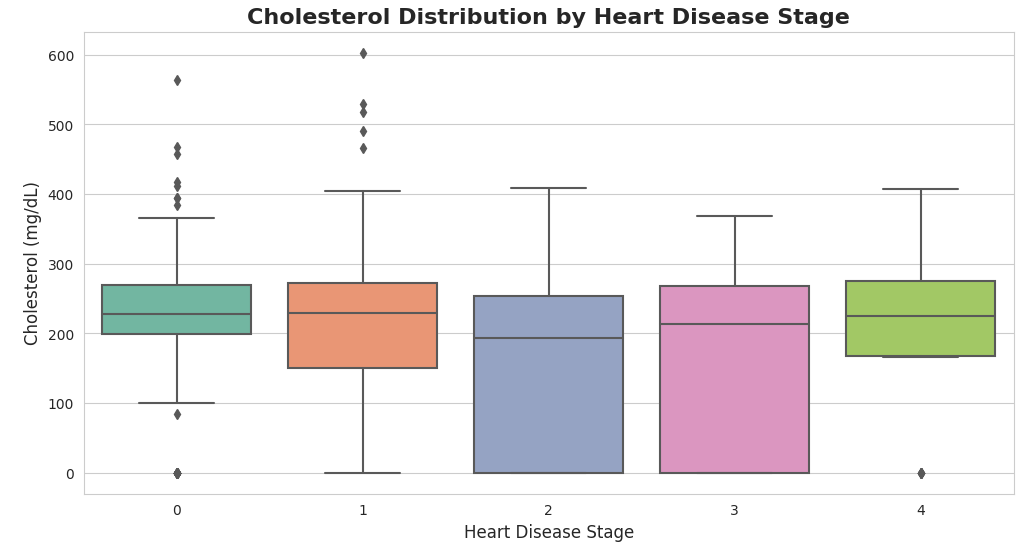
\includegraphics[width=0.85\linewidth]{serum_cholesterol_across_disease_stages.png}
  \caption{Serum cholesterol distribution across disease stages.}
  \label{fig:chol}
\end{figure}

\section{Modeling Methodology}
Data preprocessing leverages iterative imputation and z-score scaling for numerical fields, with one-hot encoding for categorical attributes. Outliers are identified using both the interquartile range (IQR) rule and an Isolation Forest ensemble to preserve explainability while curbing noise.

We benchmark Random Forest and XGBoost classifiers. The Random Forest uses 200 estimators, maximum depth 8, and class-balanced weighting, while XGBoost applies learning-rate 0.05, maximum depth 4, subsample 0.8, and column subsample 0.8. Five-fold stratified cross-validation tunes hyperparameters and calibrates predicted probabilities through Platt scaling. Shapley value decomposition further validates the clinical plausibility of dominant features such as chest pain type, ST depression (\textit{oldpeak}), number of affected vessels (\textit{ca}), and thalassemia status.

\section{System Architecture and Security Controls}
Heartlytics couples predictive analytics with secure-by-design workflows. Figure~\ref{fig:topology} illustrates the macro-level deployment topology, while Figure~\ref{fig:encryption} details the envelope encryption workflow safeguarding both data at rest and in transit.

\begin{figure}[t]
  \centering
  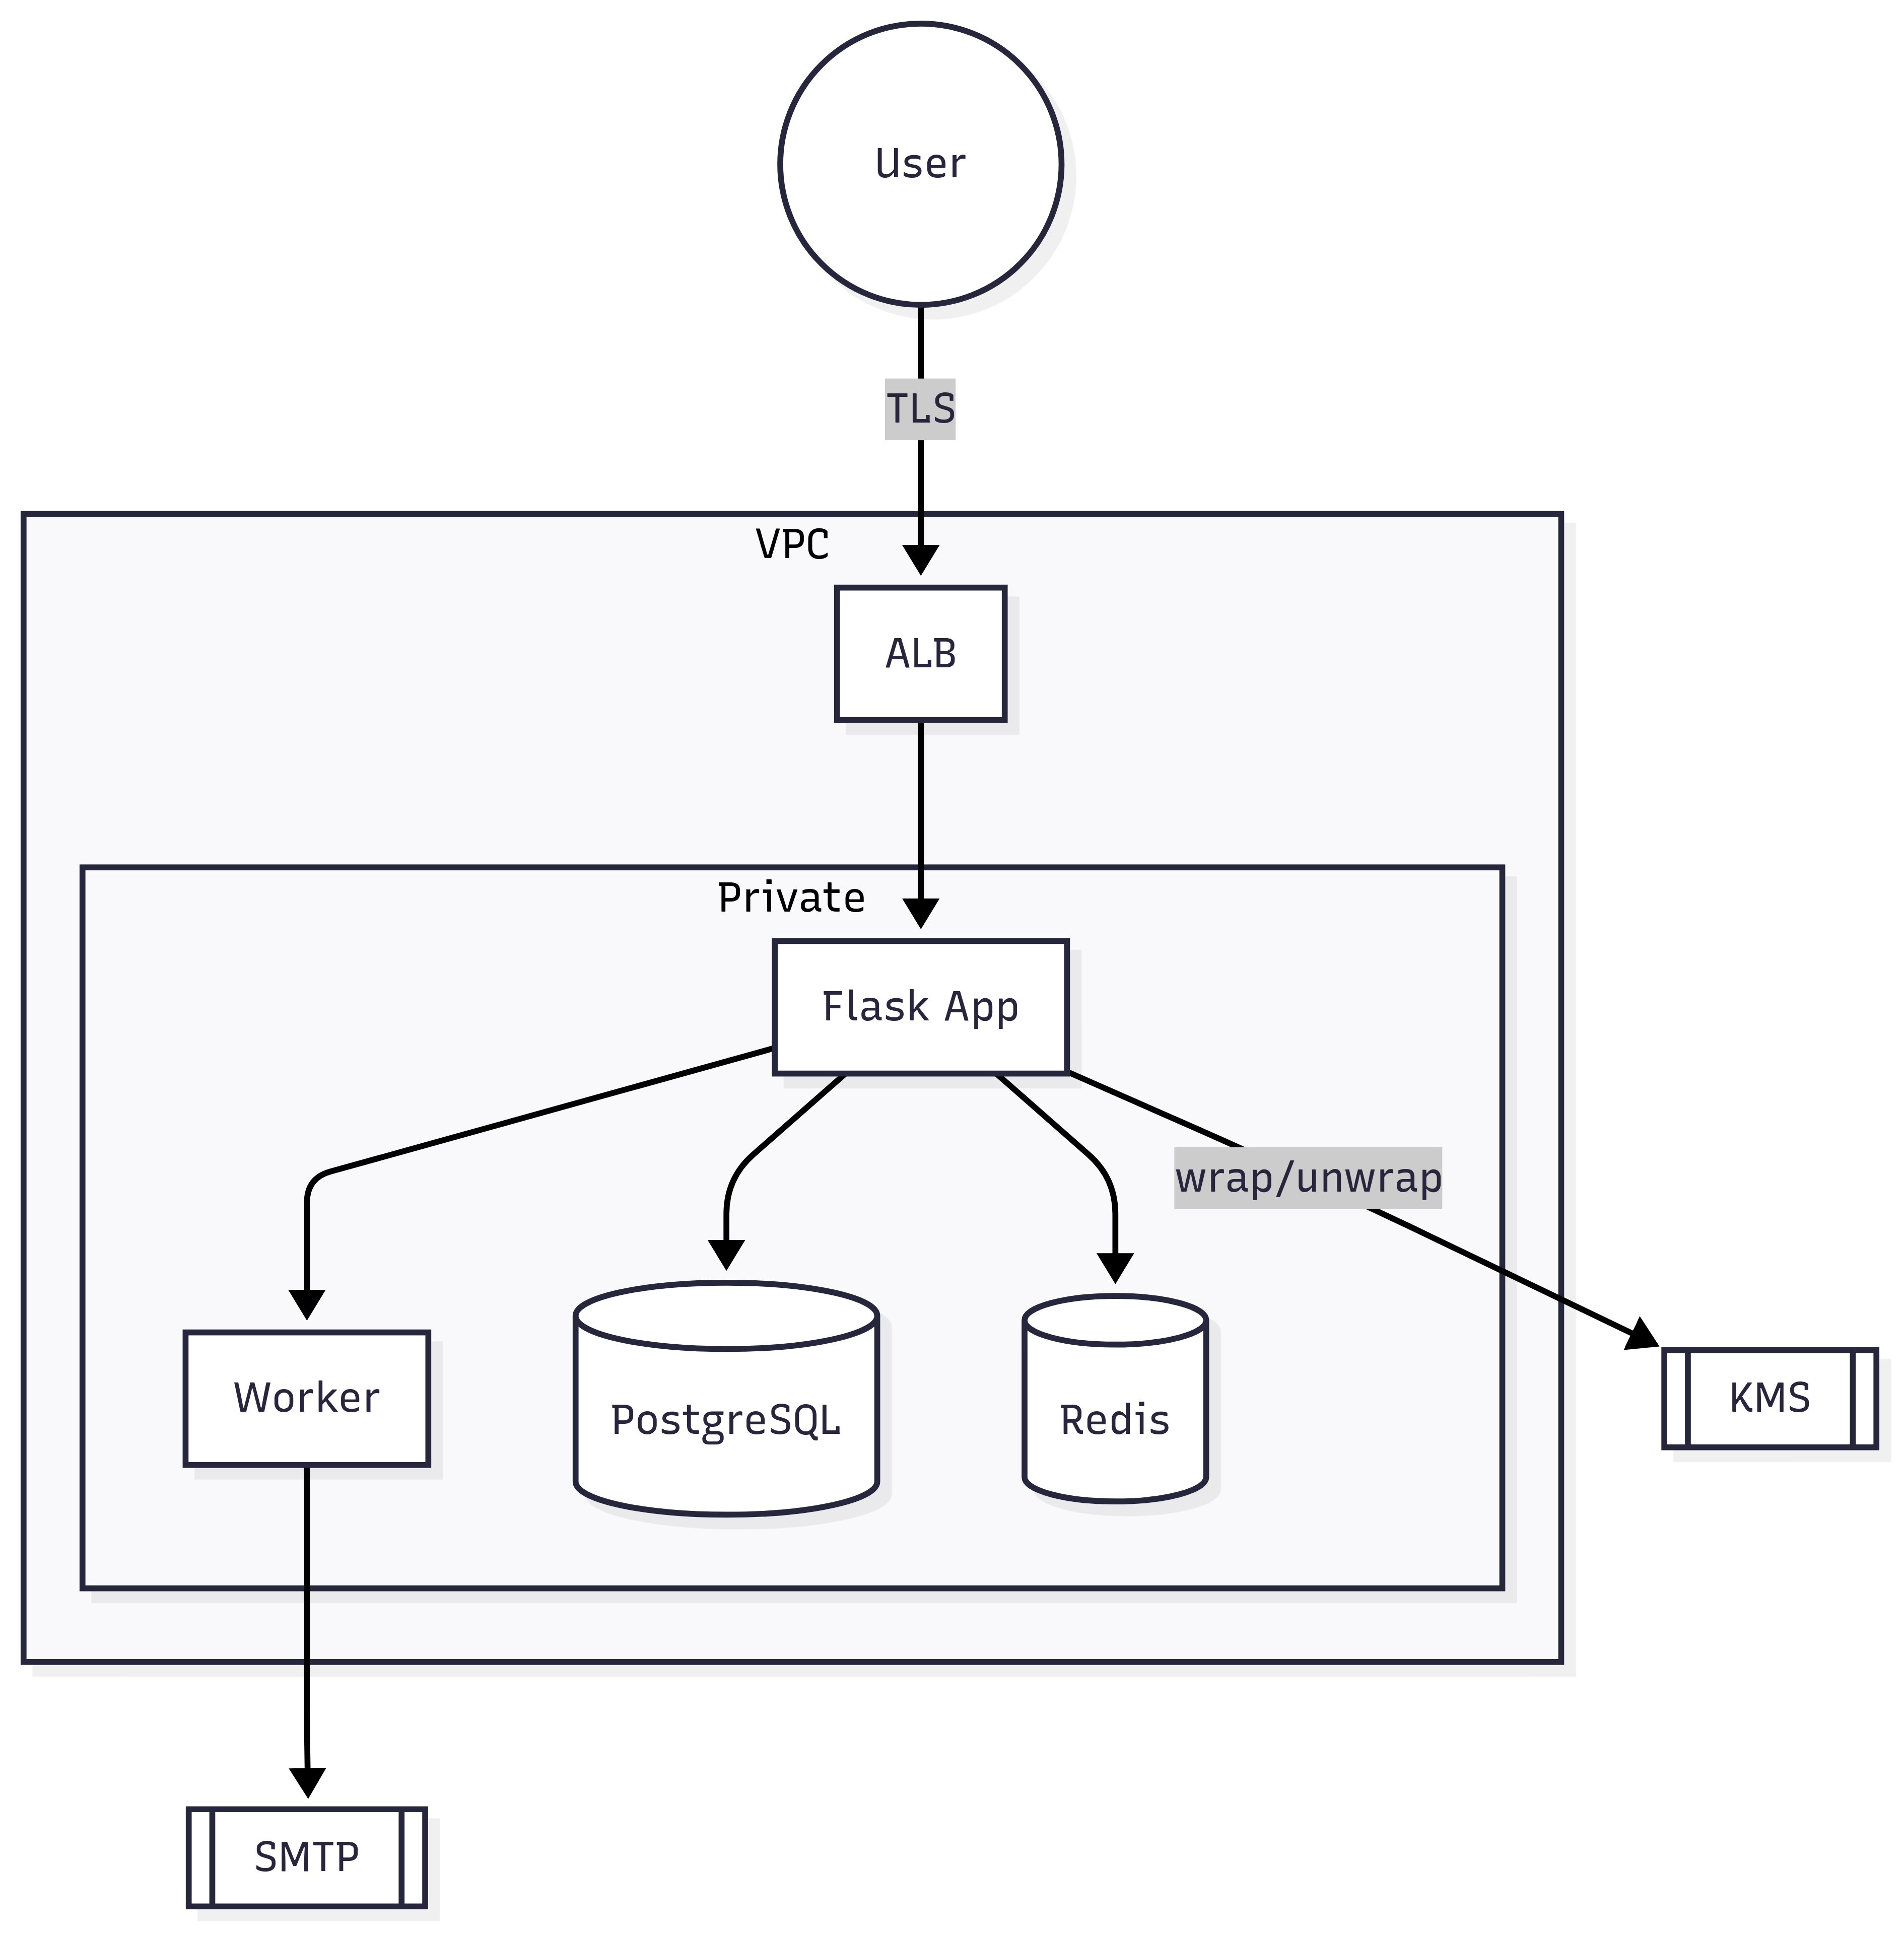
\includegraphics[width=0.9\linewidth]{deployment_topology.png}
  \caption{High-level deployment topology of the Heartlytics platform.}
  \label{fig:topology}
\end{figure}

\begin{figure}[t]
  \centering
  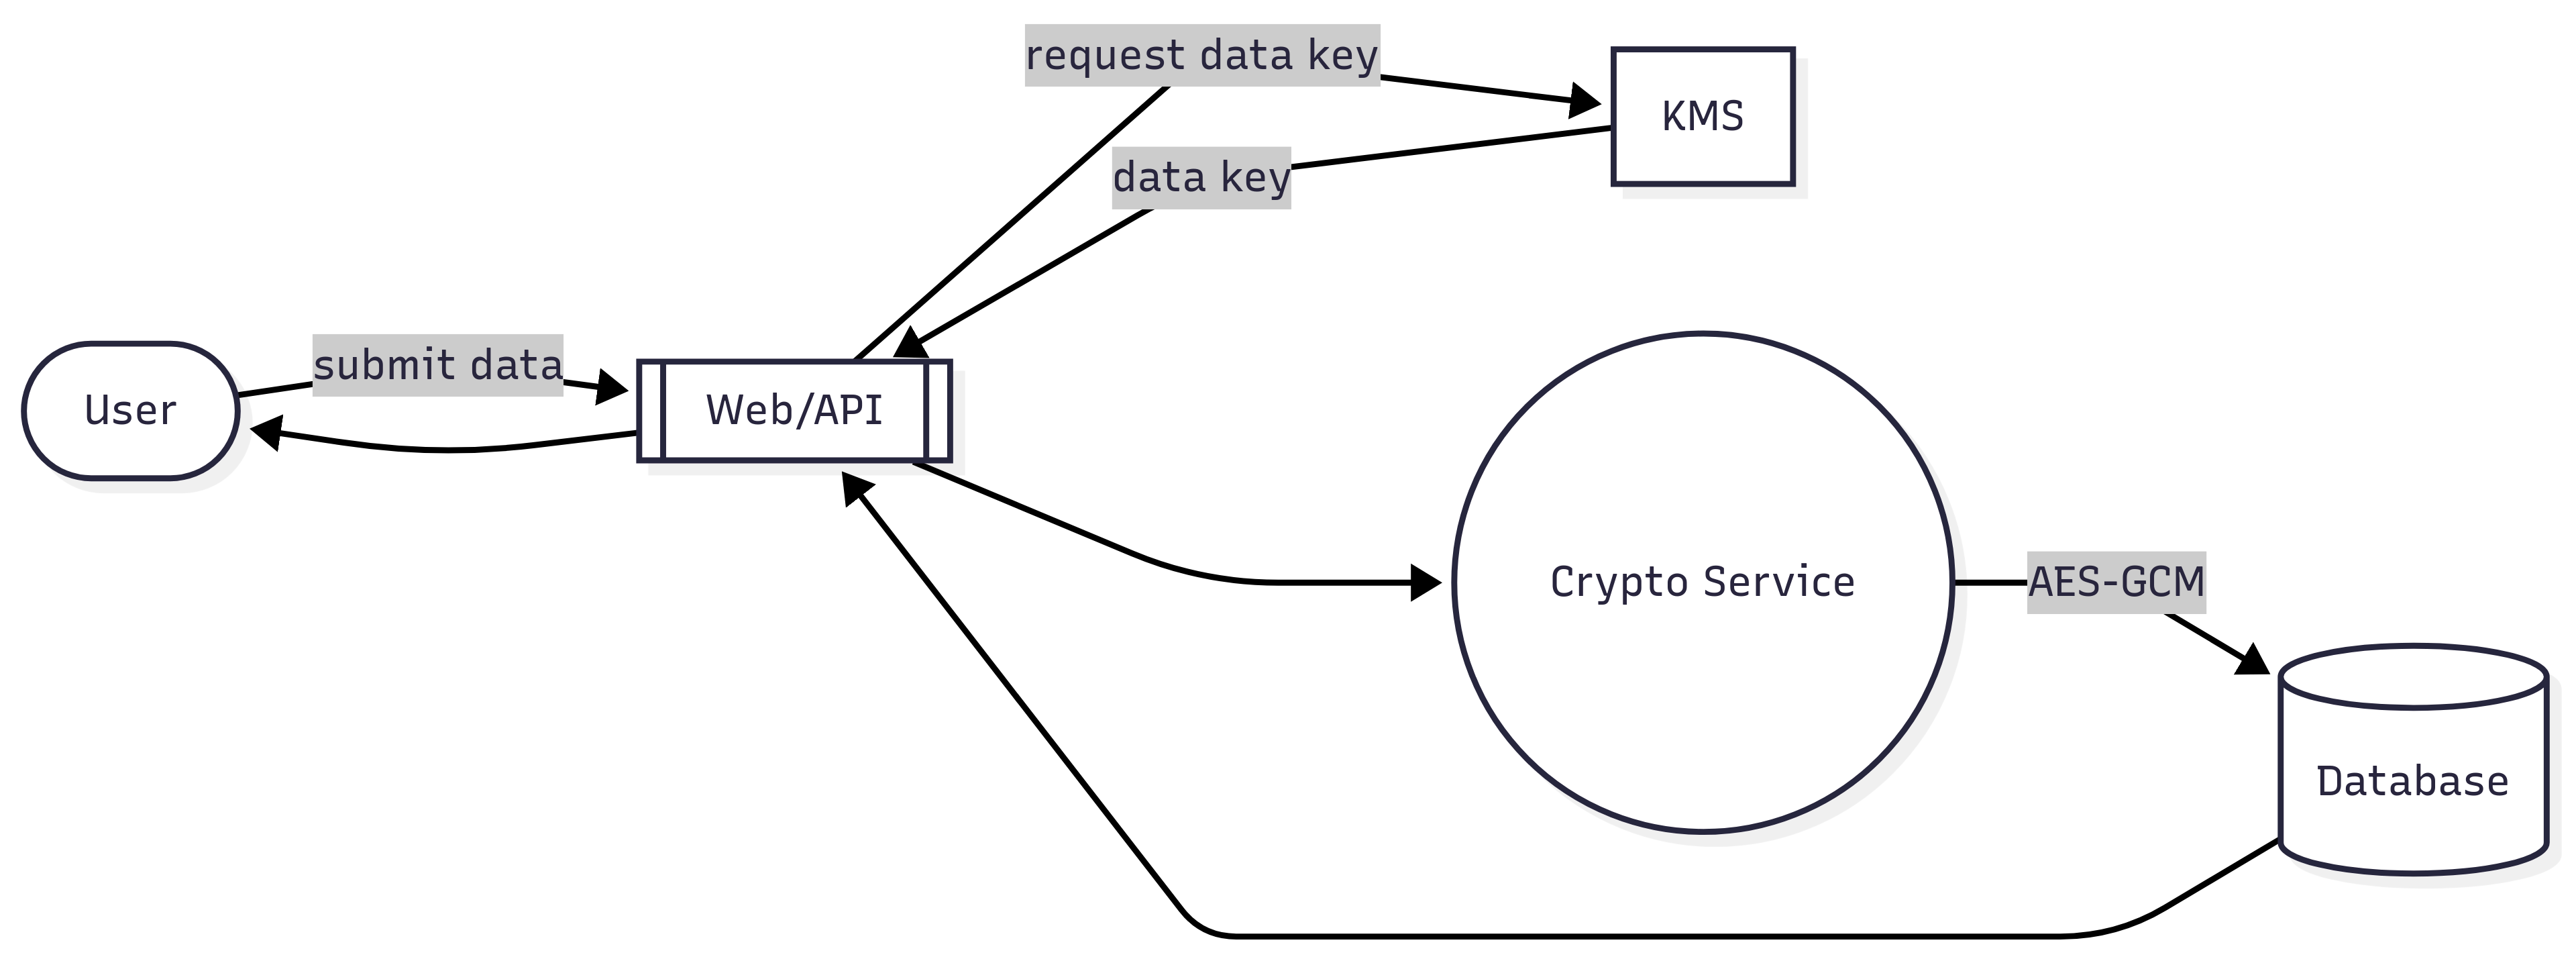
\includegraphics[width=0.9\linewidth]{envelope_encryption_workflow.png}
  \caption{Envelope encryption workflow protecting model artifacts and secrets.}
  \label{fig:encryption}
\end{figure}

Complementing the infrastructure view, Figures~\ref{fig:c4_context}--\ref{fig:c4_components} provide the full C4 stack, mapping external actors, logical containers, and component boundaries that orchestrate ingestion, model serving, and observability.

\begin{figure}[t]
  \centering
  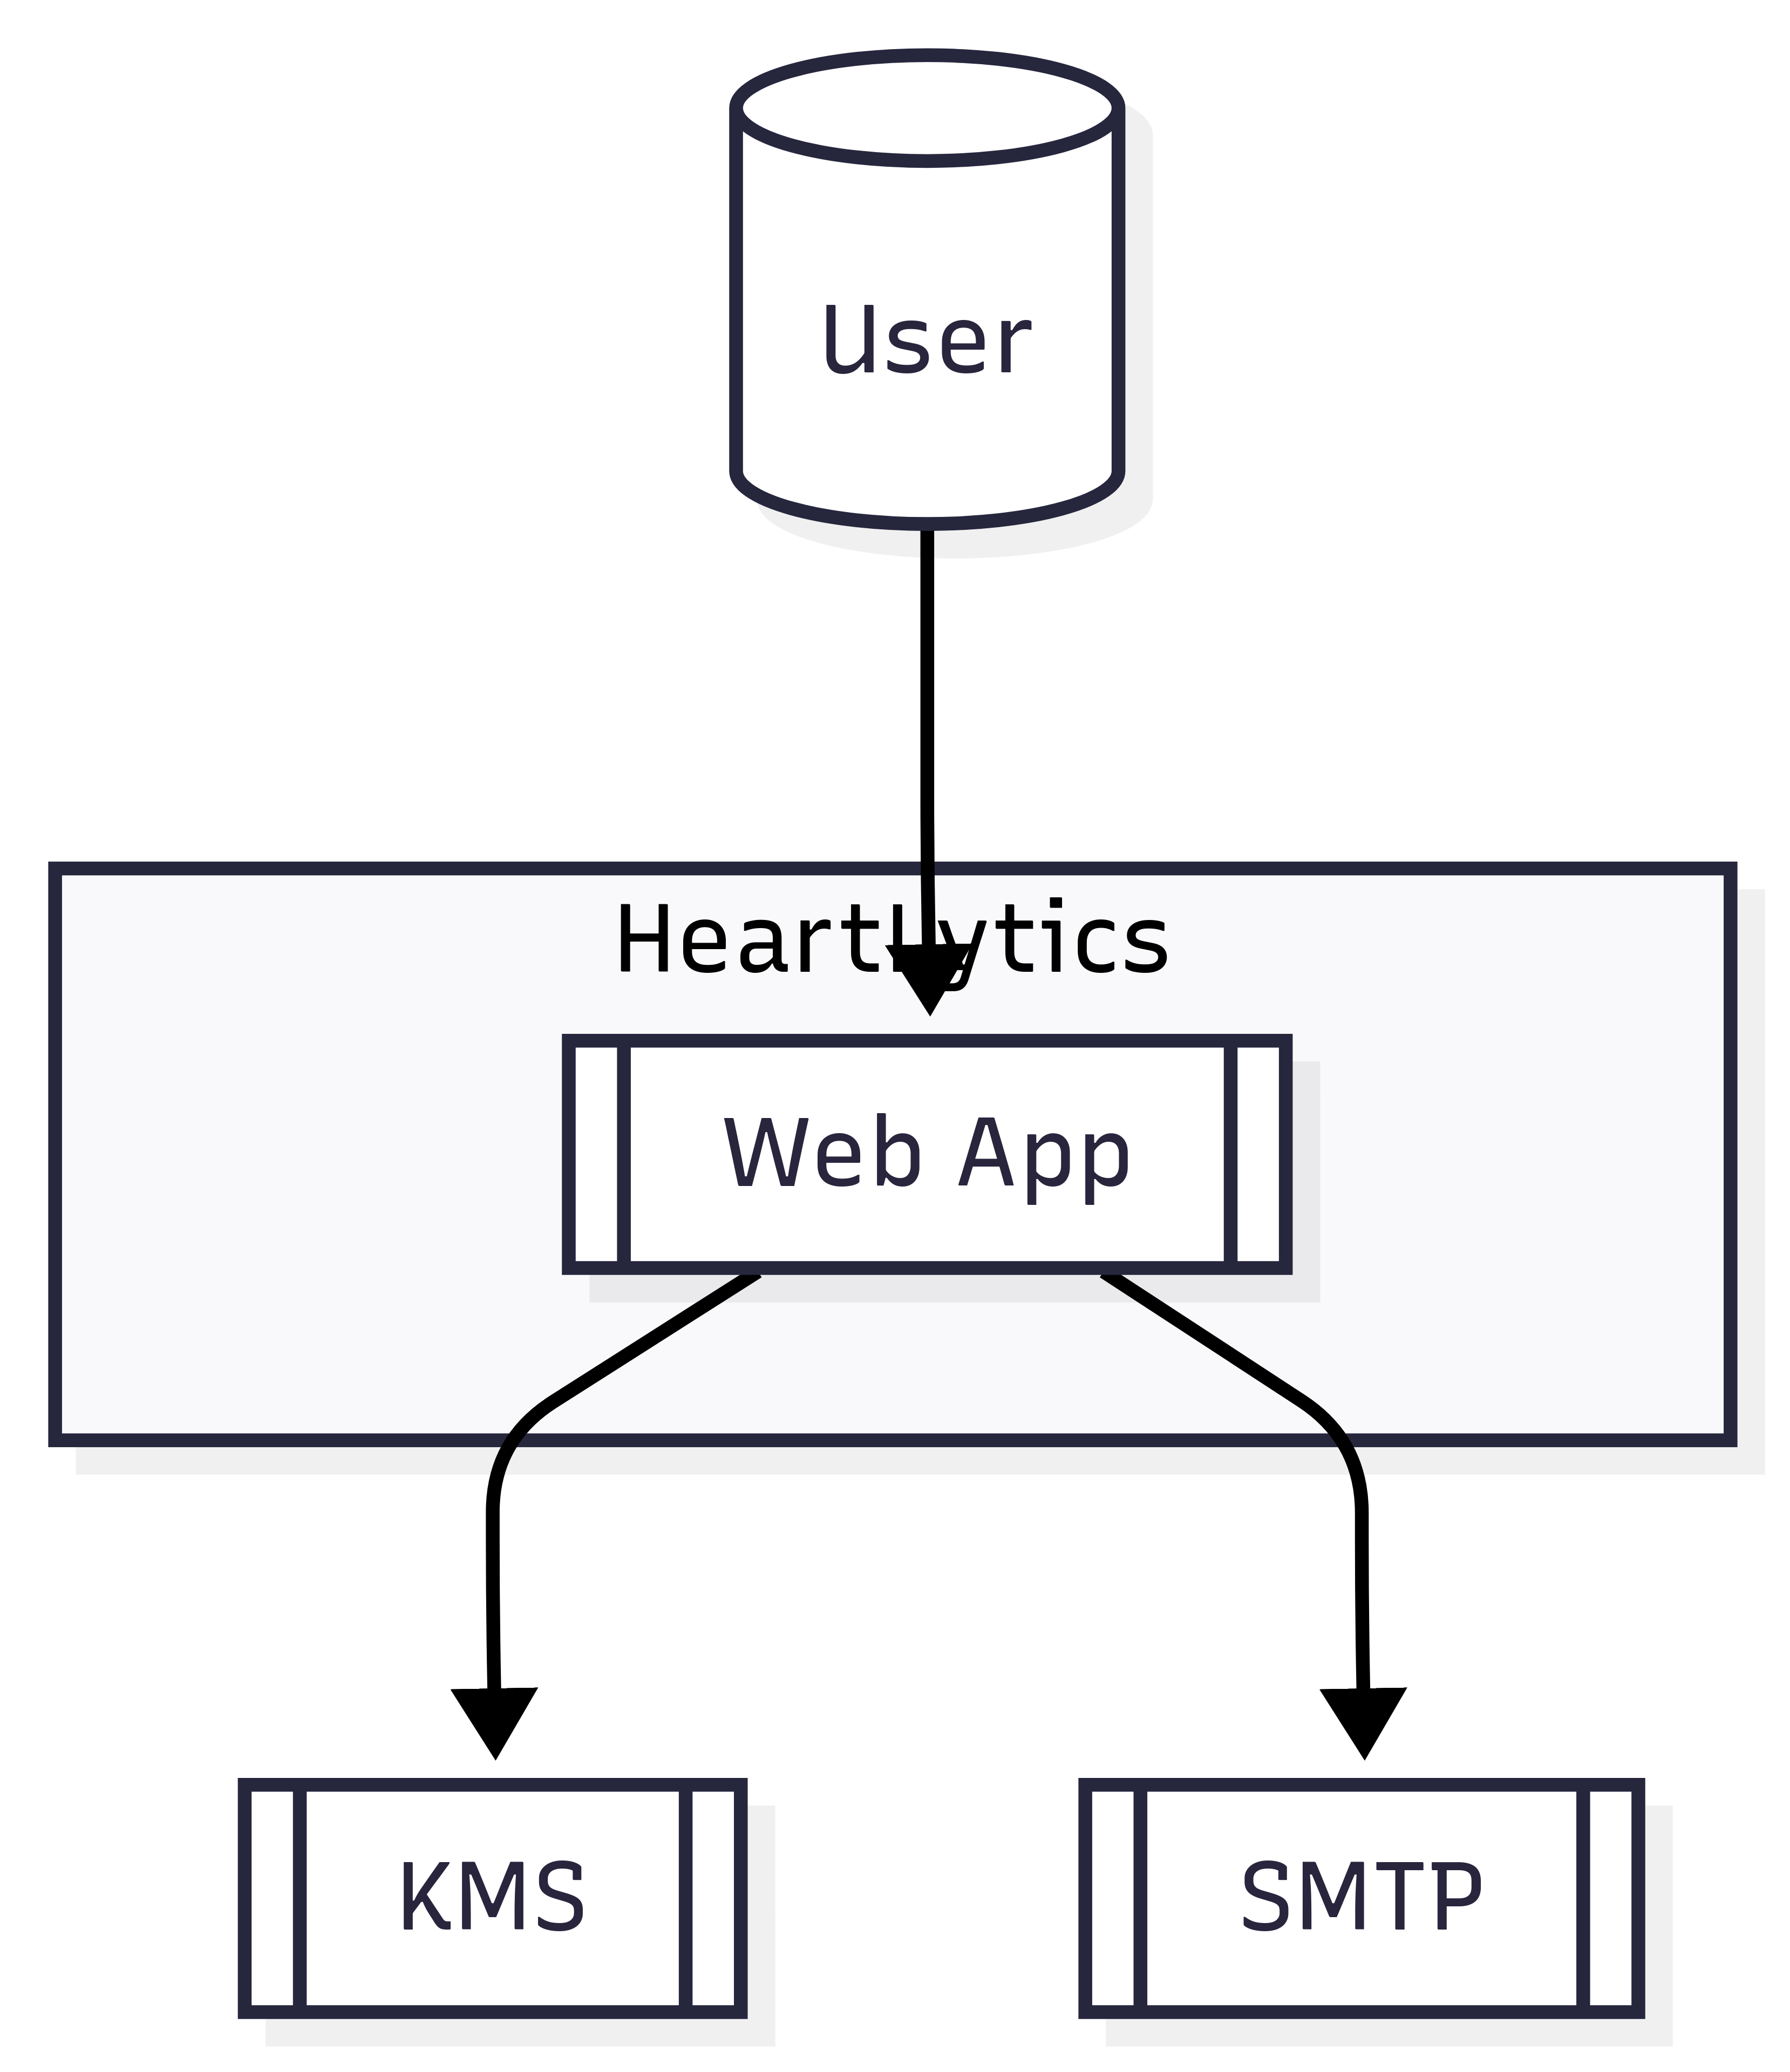
\includegraphics[width=0.9\linewidth]{c4_level_1_context.png}
  \caption{C4 Level~1 context view situating Heartlytics among external actors and SaaS dependencies.}
  \label{fig:c4_context}
\end{figure}

\begin{figure}[t]
  \centering
  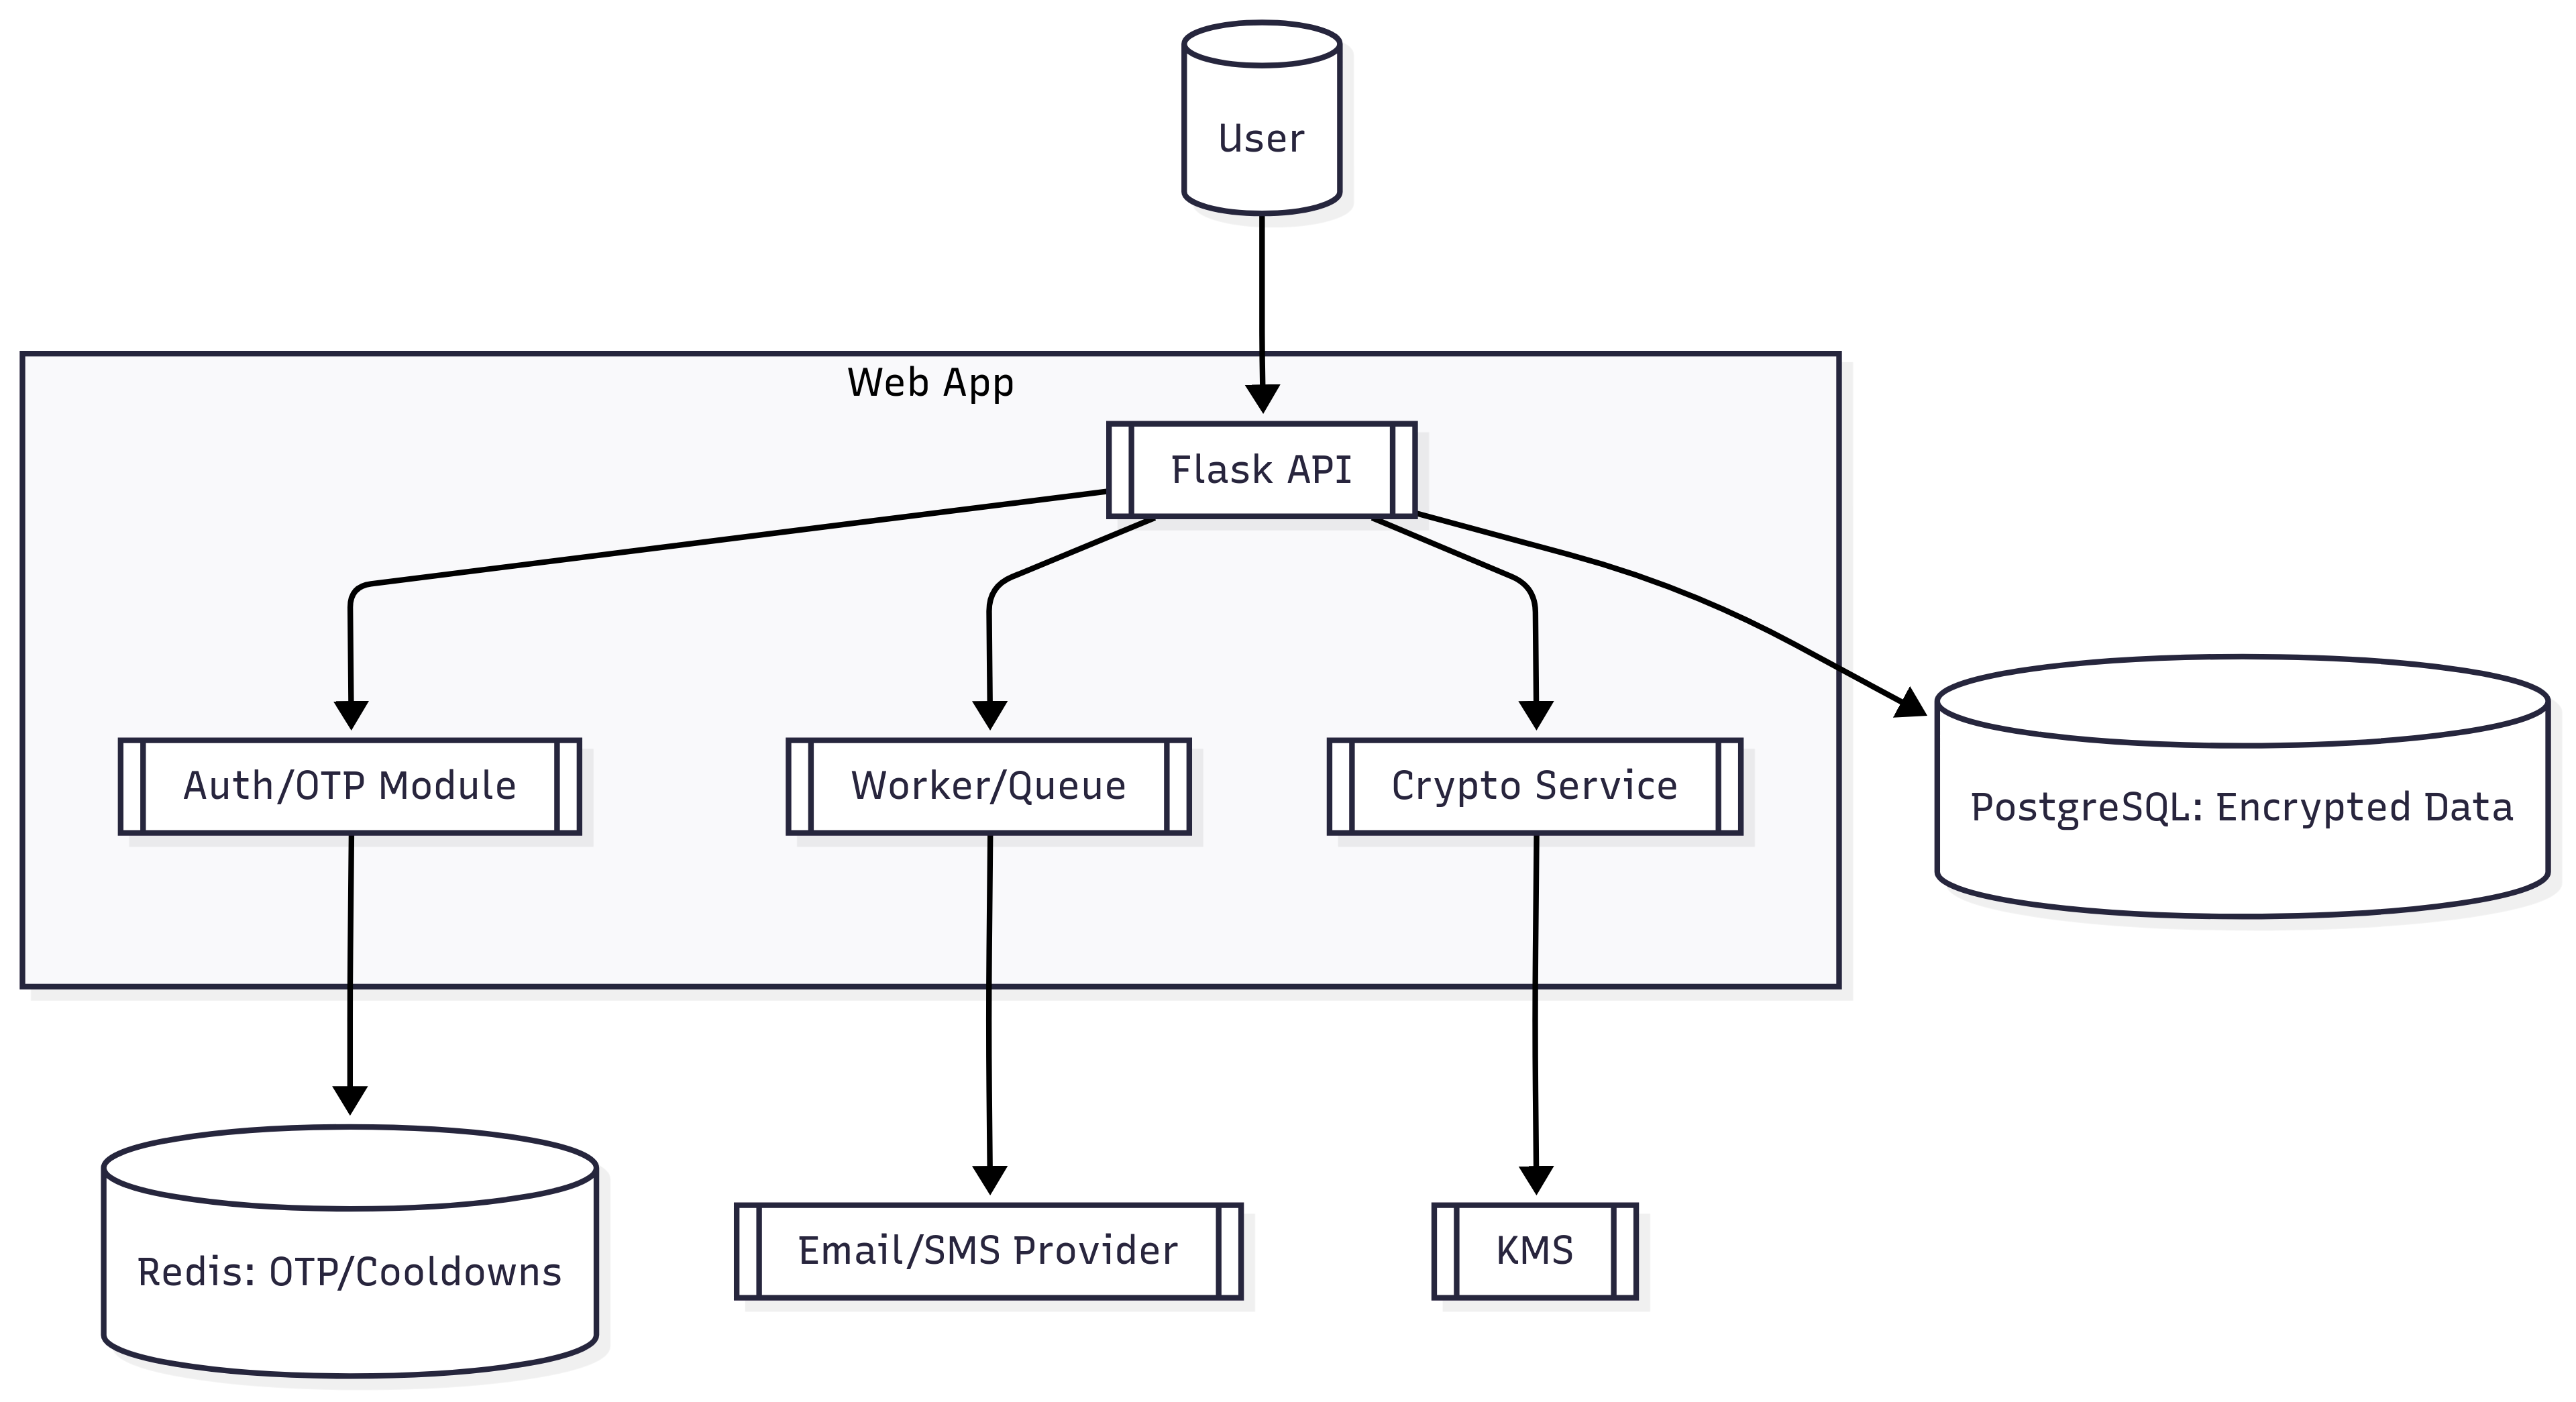
\includegraphics[width=0.9\linewidth]{c4_level_2_containers.png}
  \caption{C4 Level~2 container diagram outlining web, API, model-serving, and analytics services.}
  \label{fig:c4_containers}
\end{figure}

\begin{figure}[t]
  \centering
  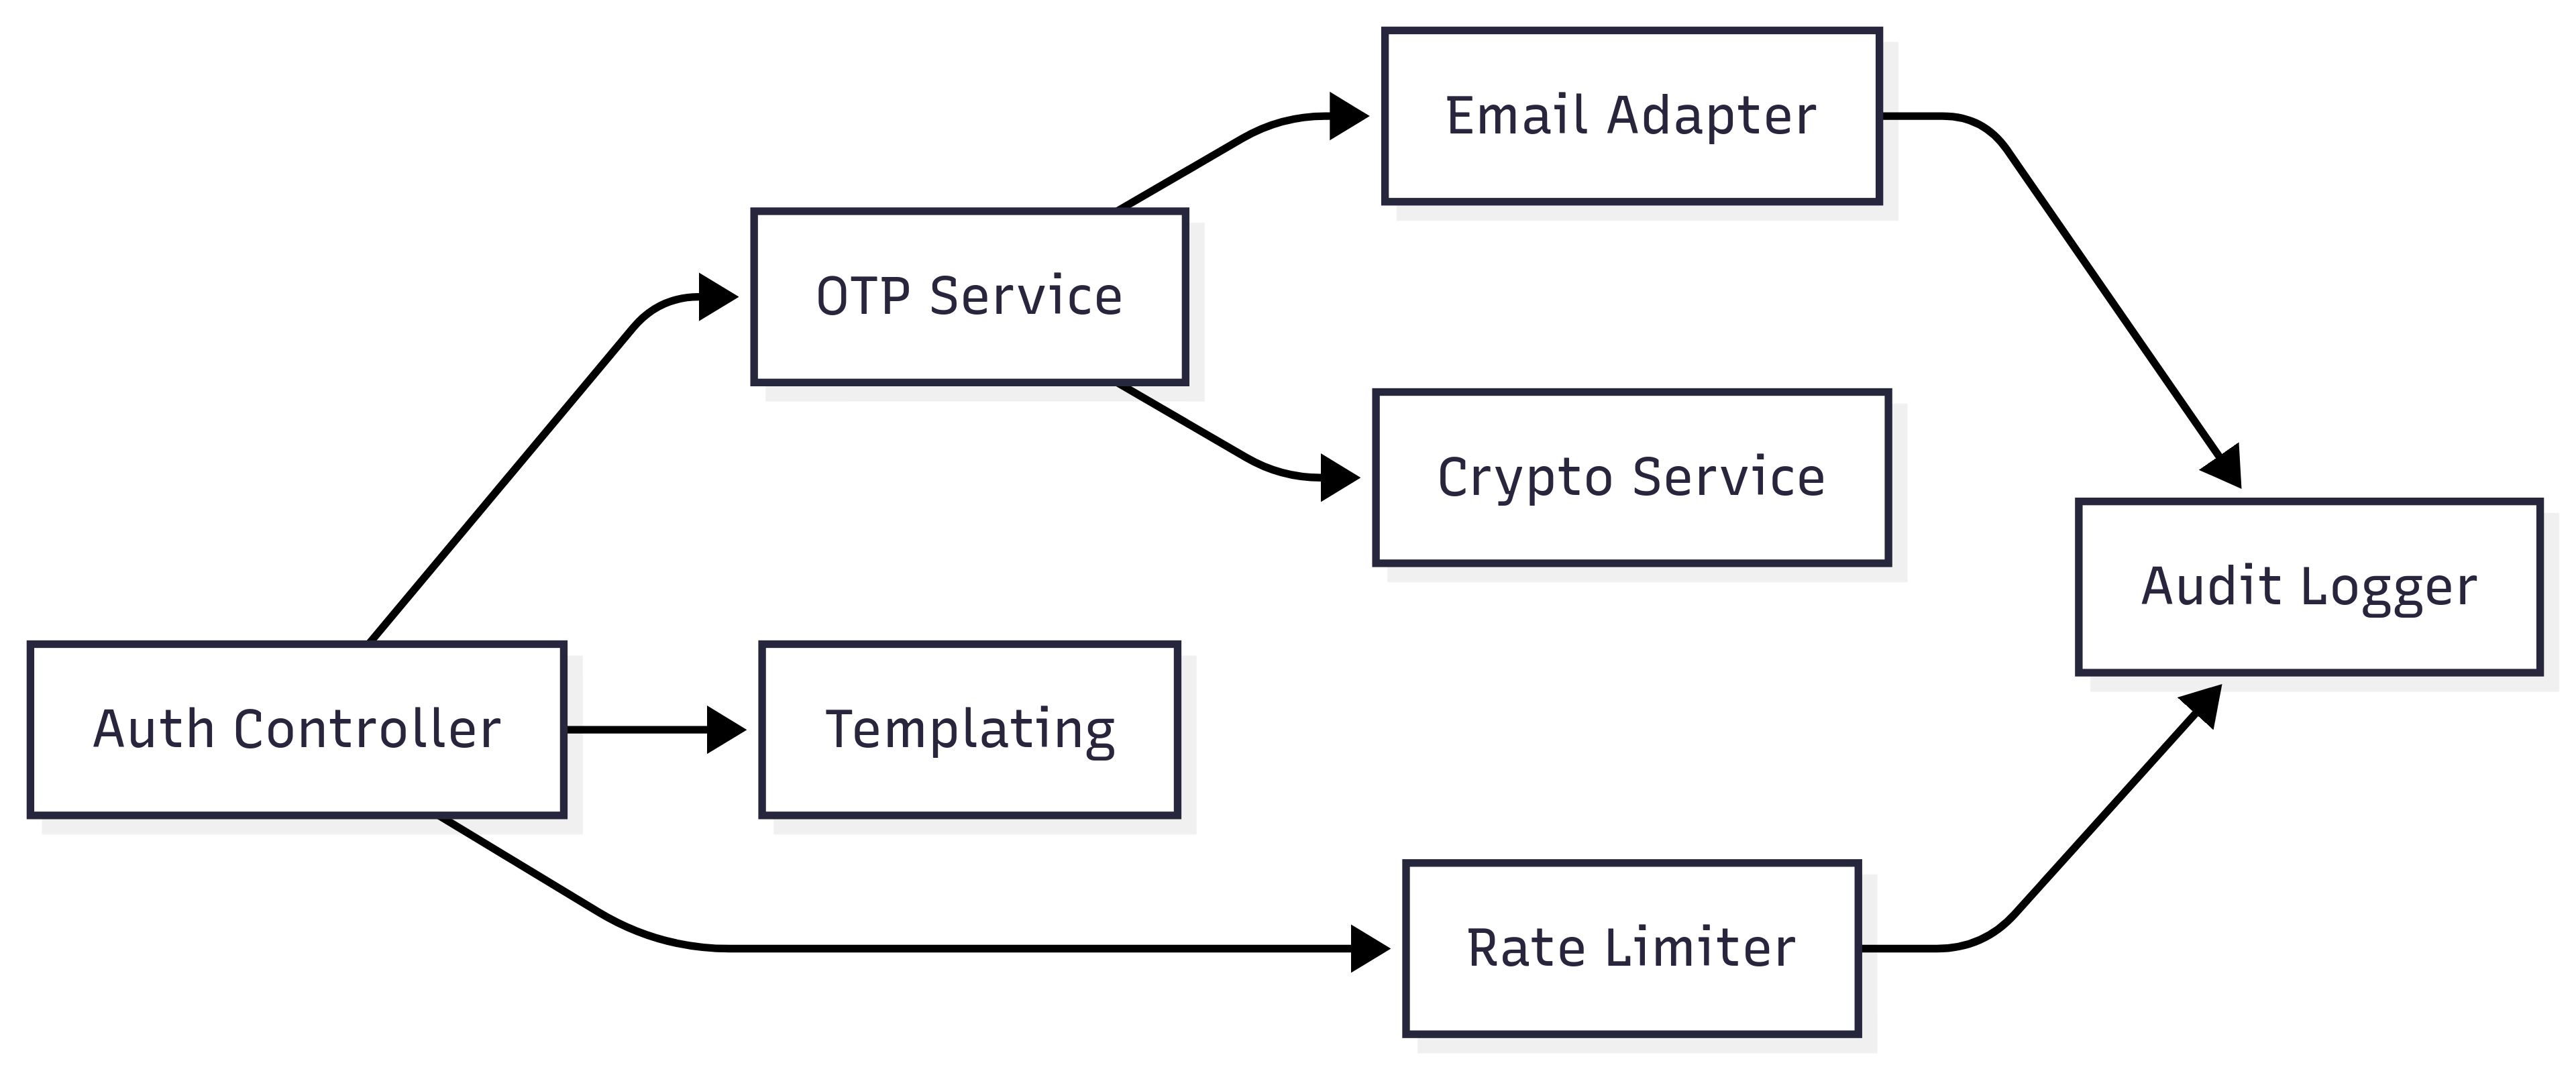
\includegraphics[width=0.9\linewidth]{c4_level_3_components.png}
  \caption{C4 Level~3 component view detailing intra-application modules and shared libraries.}
  \label{fig:c4_components}
\end{figure}

The layered blueprint in Figure~\ref{fig:system_arch} and the security automation overlay in Figure~\ref{fig:security_automation} align infrastructure tiers with monitoring, CI/CD, and secret-rotation guardrails. Figure~\ref{fig:database_erd} documents relational entities supporting traceable predictions, while Figure~\ref{fig:rbac} summarizes the role-based access controls governing user privileges.

\begin{figure}[t]
  \centering
  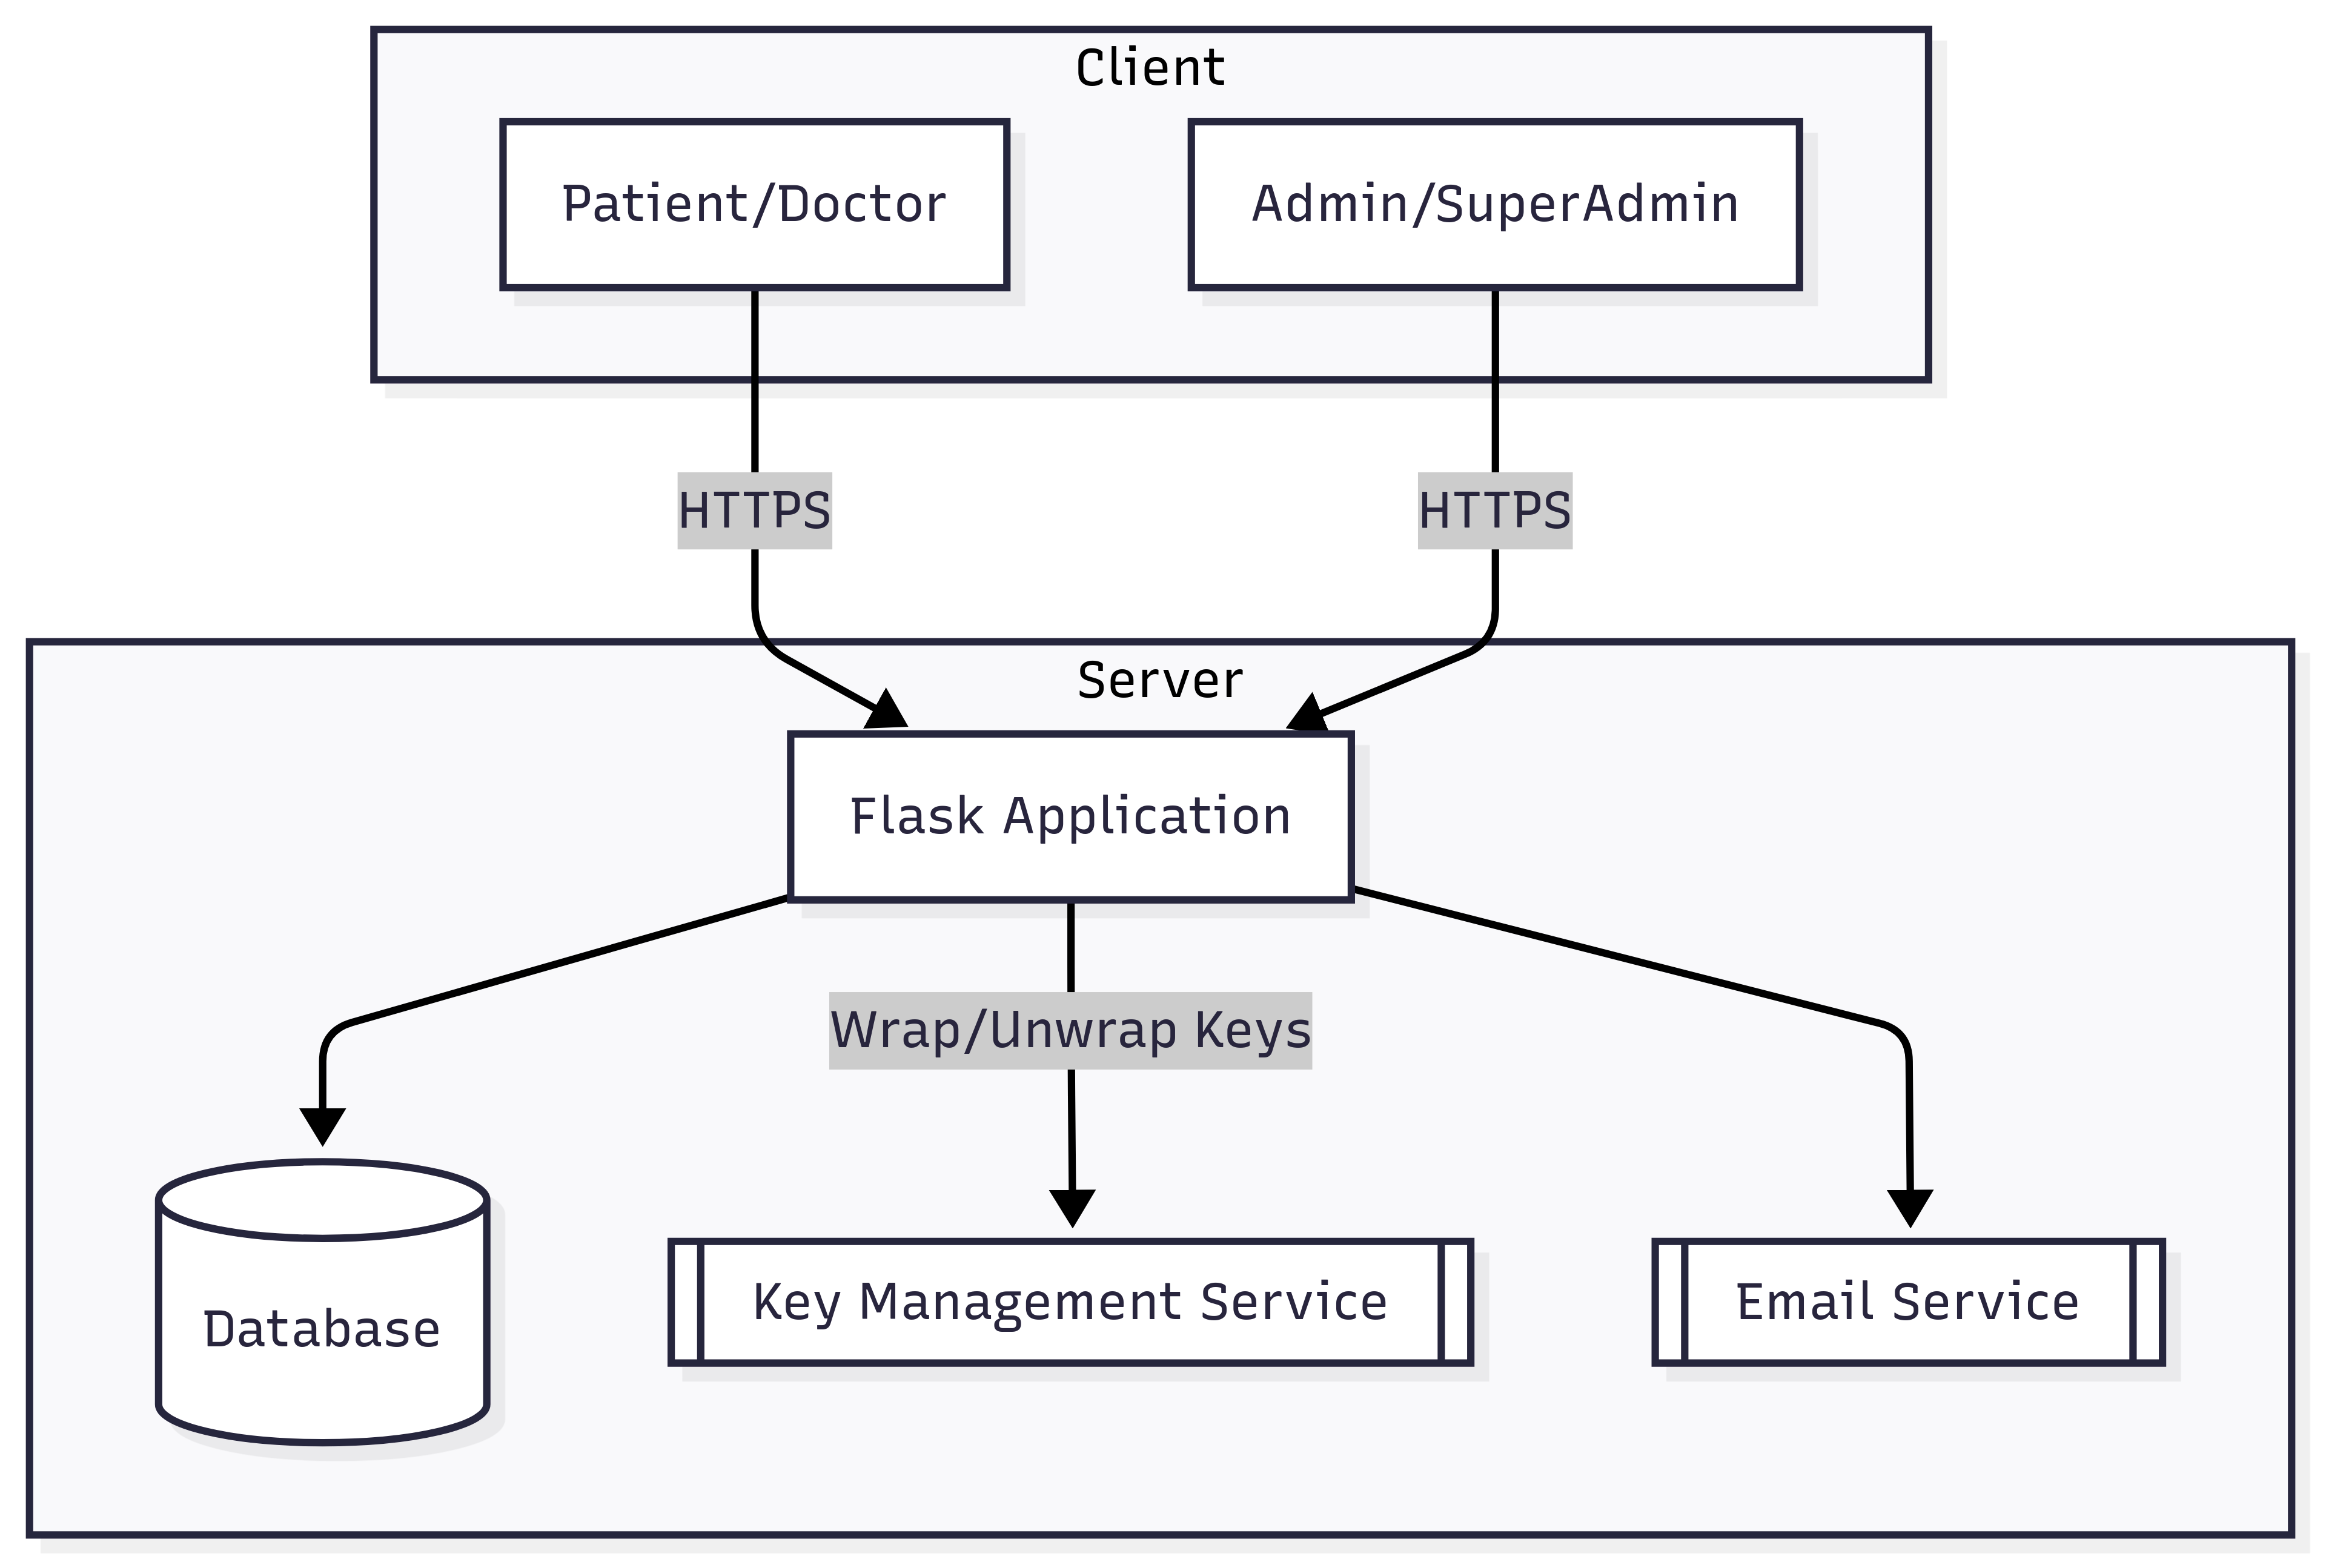
\includegraphics[width=0.9\linewidth]{high_level_system_architecture.png}
  \caption{High-level system architecture mapping client channels to platform services and data stores.}
  \label{fig:system_arch}
\end{figure}

\begin{figure}[t]
  \centering
  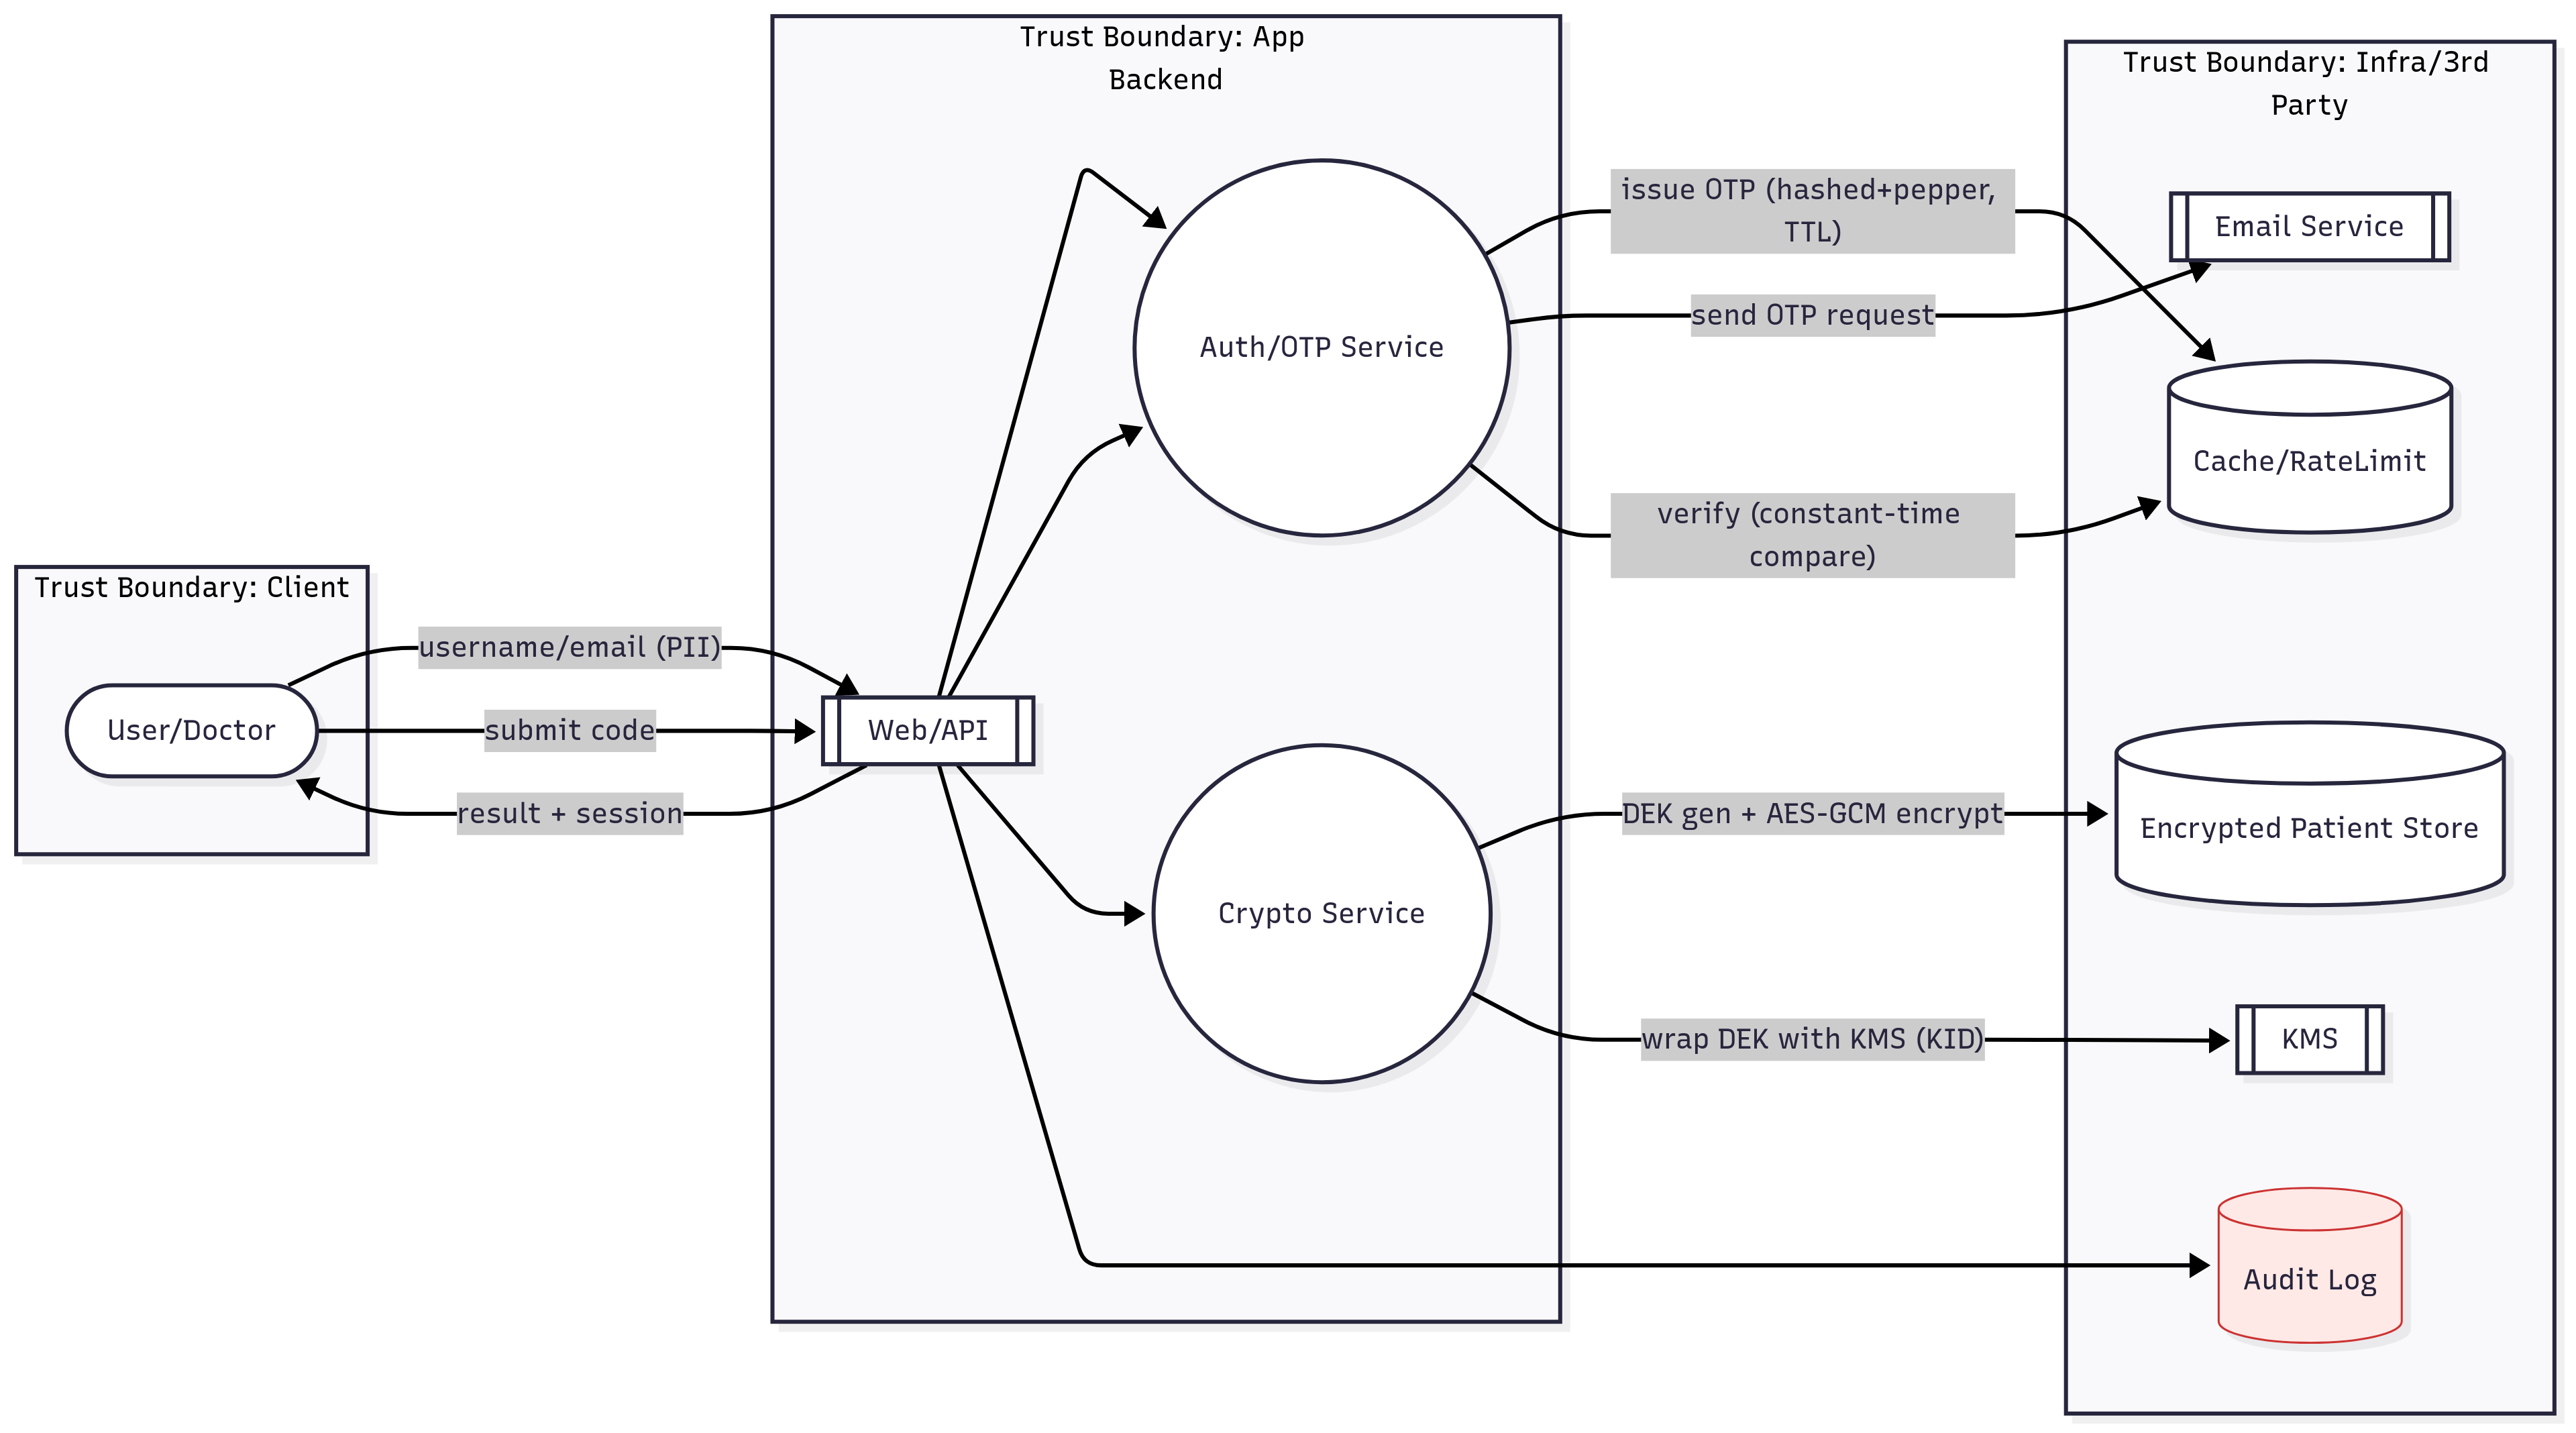
\includegraphics[width=0.9\linewidth]{sa.png}
  \caption{Security automation roadmap coordinating monitoring, incident response, and compliance activities.}
  \label{fig:security_automation}
\end{figure}

\begin{figure}[t]
  \centering
  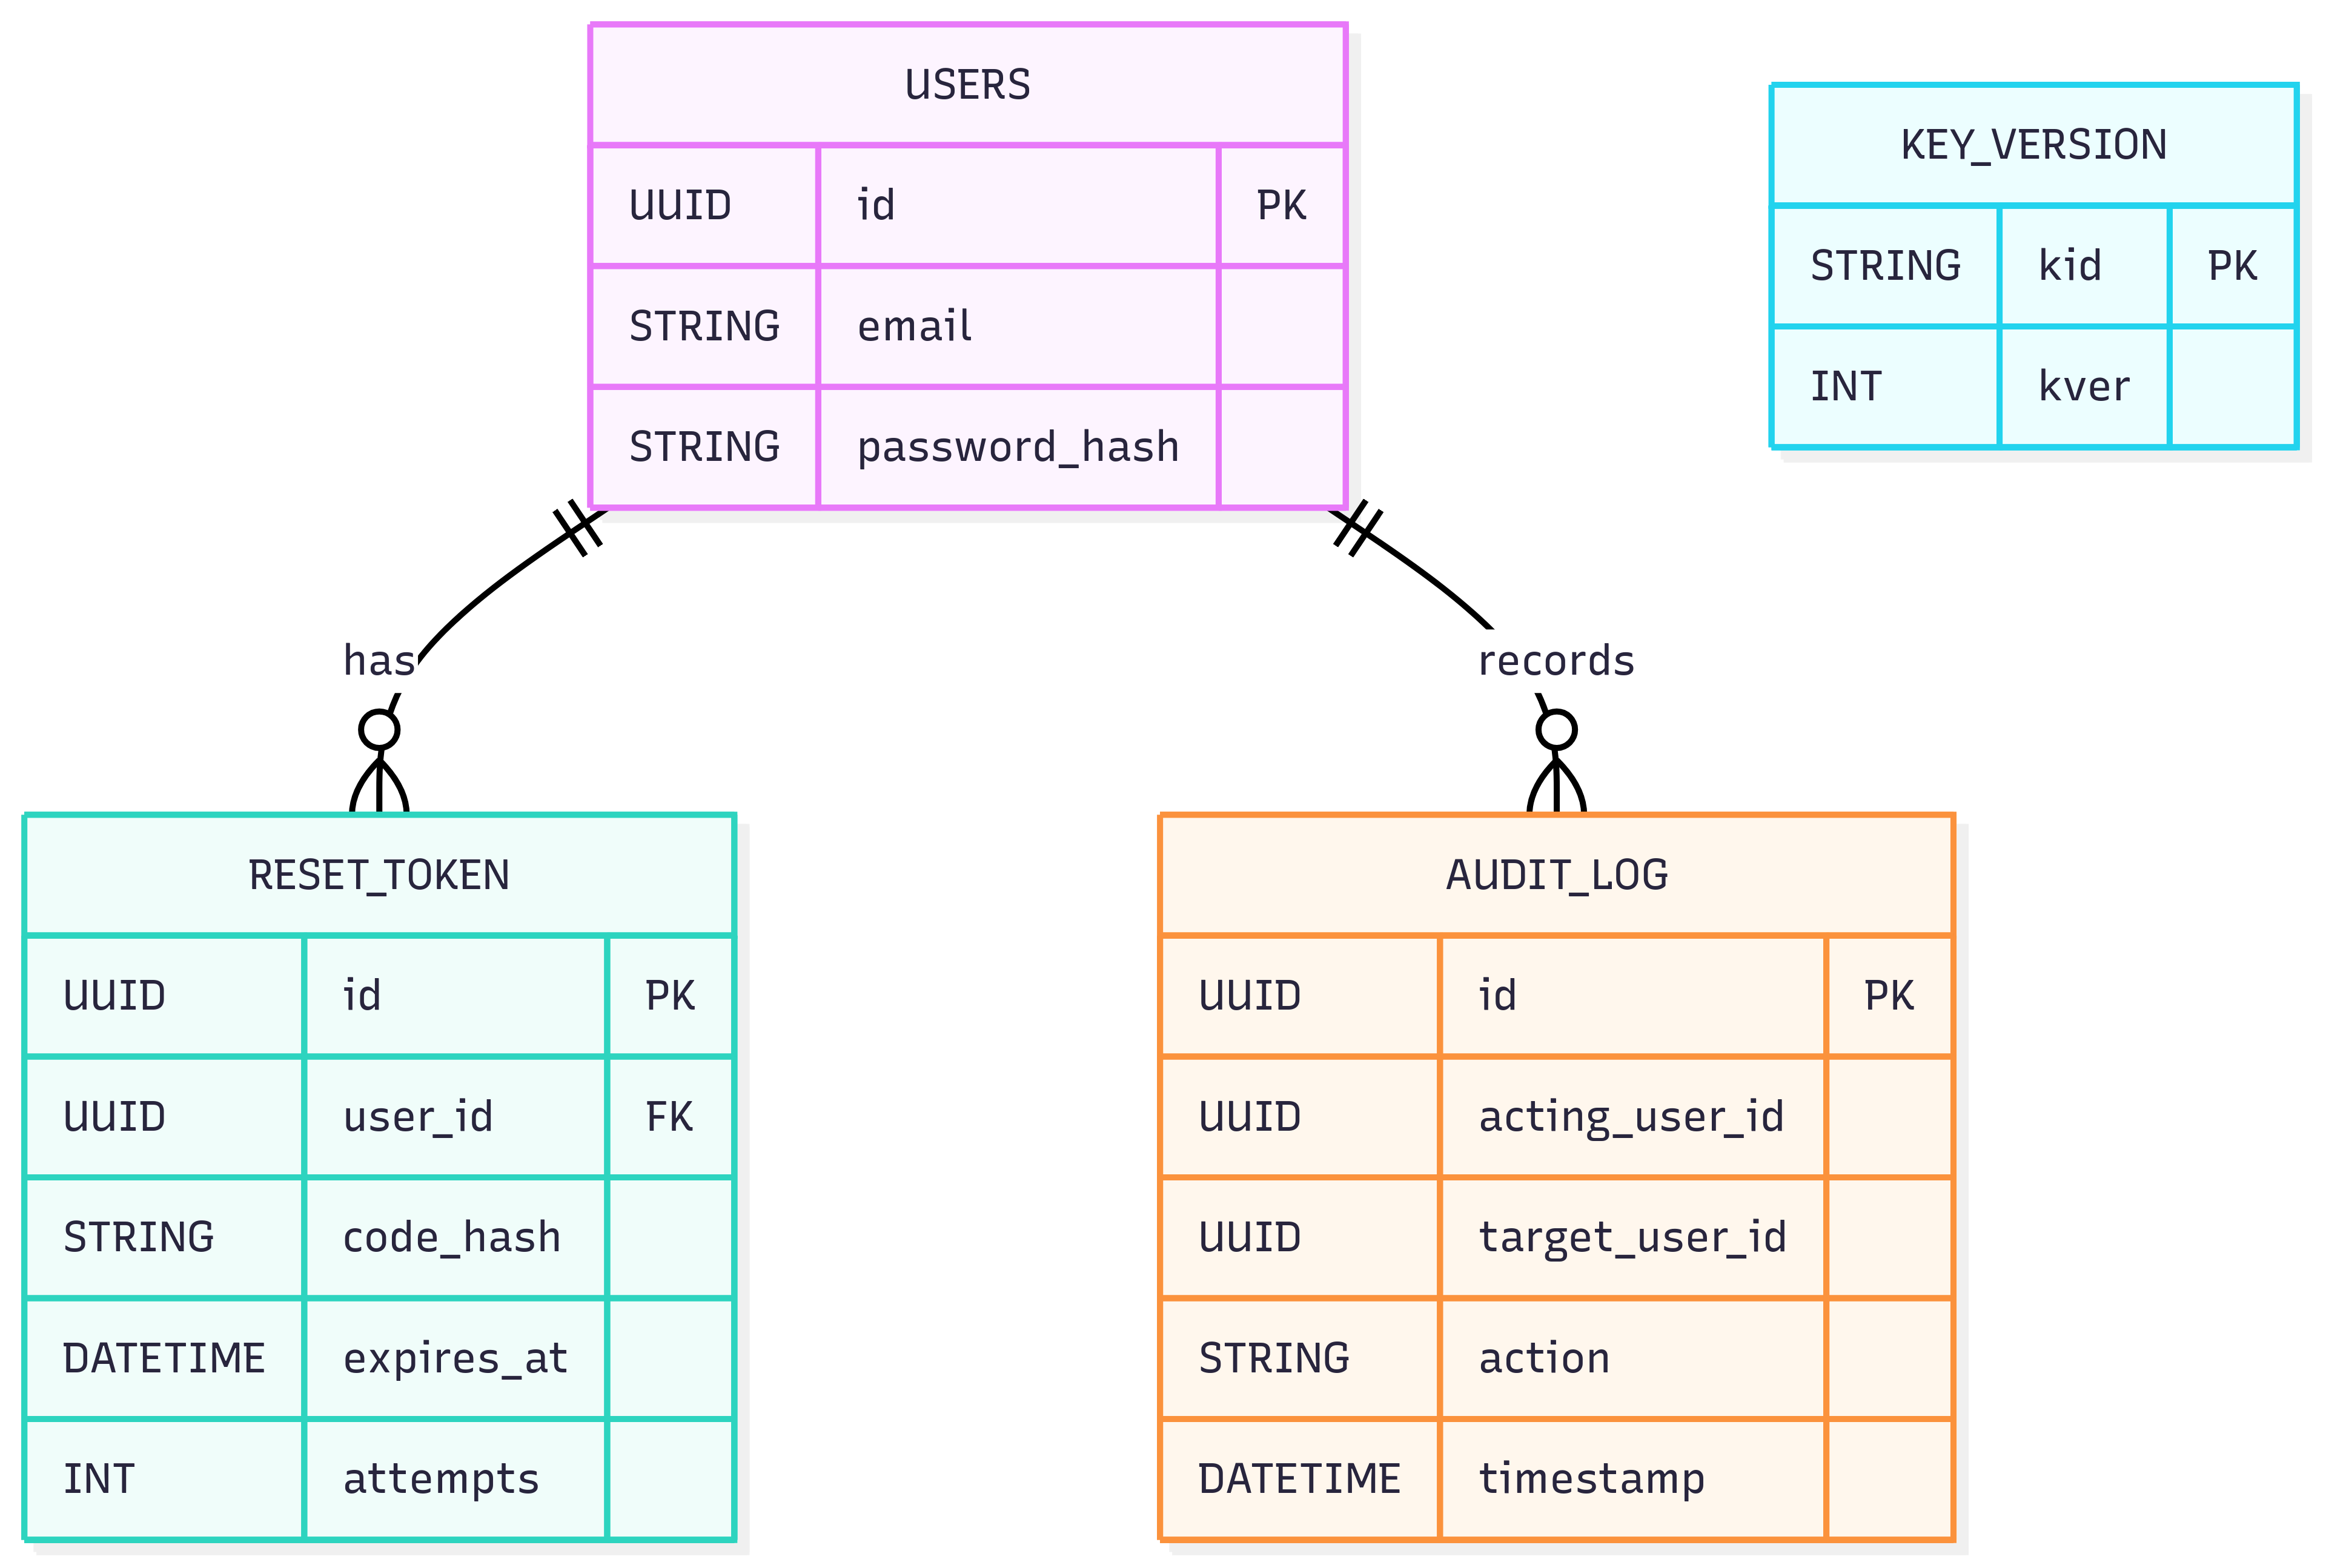
\includegraphics[width=0.9\linewidth]{database_erd.png}
  \caption{Entity-relationship diagram (ERD) capturing patient, prediction, audit, and policy metadata stores.}
  \label{fig:database_erd}
\end{figure}

\begin{figure}[t]
  \centering
  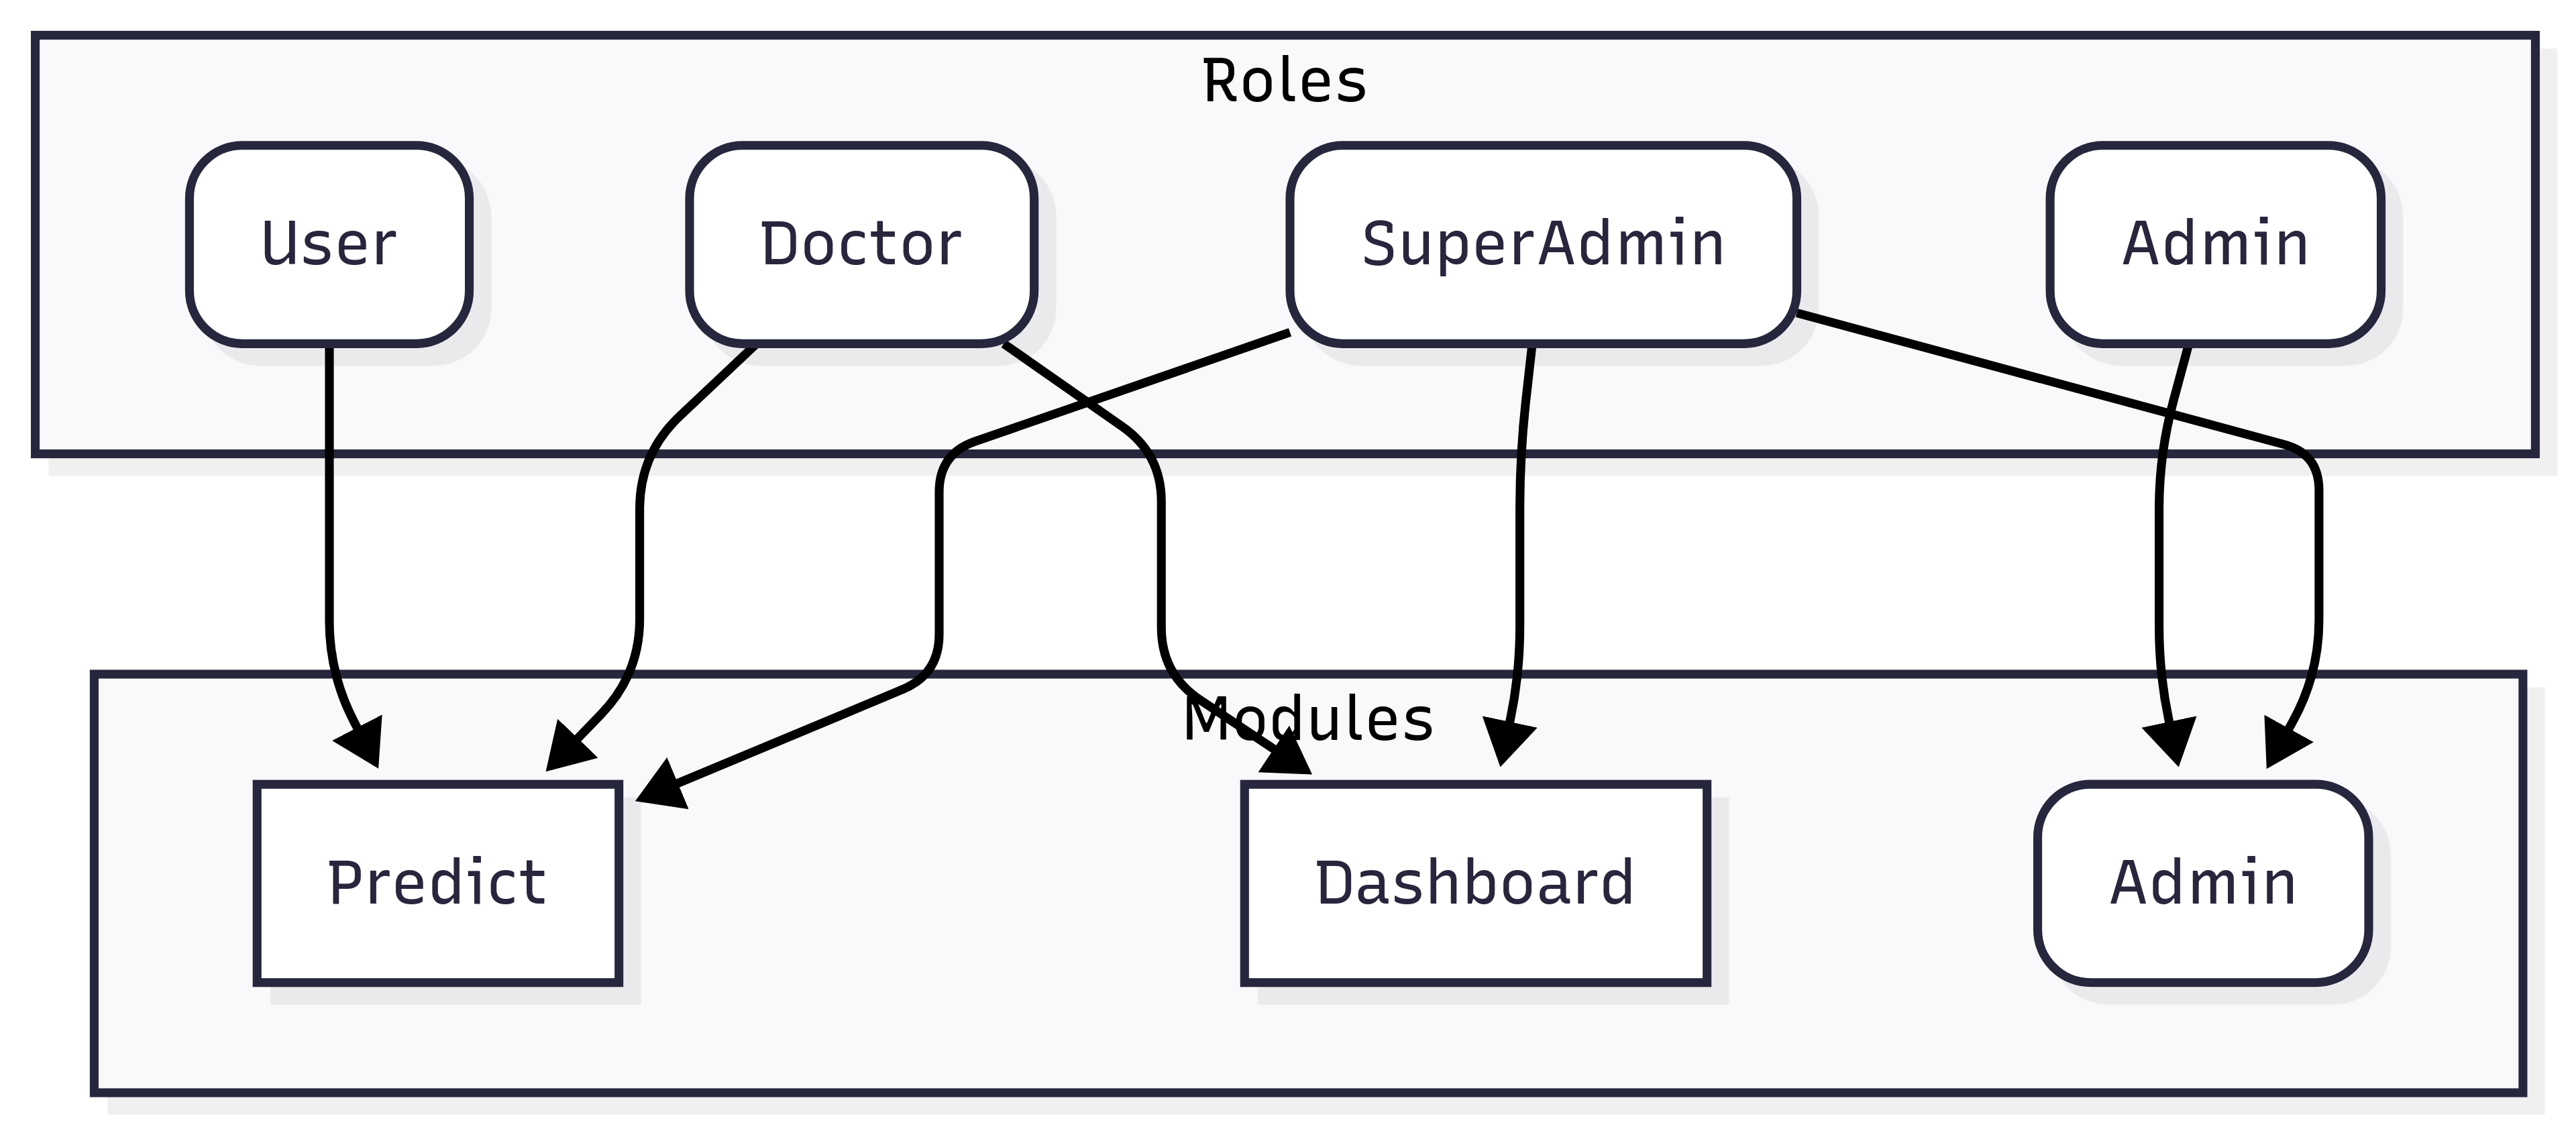
\includegraphics[width=0.85\linewidth]{role_based_access_control_rbac.png}
  \caption{Role-based access control matrix assigning permissions to Users, Doctors, Admins, and SuperAdmins.}
  \label{fig:rbac}
\end{figure}

Security-aware flows (Figures~\ref{fig:security_flow}--\ref{fig:sequence_interactions}) trace data-at-rest protections, threat mitigations, and service-to-service exchanges, ensuring encryption coverage and explicit trust boundaries.

\begin{figure}[t]
  \centering
  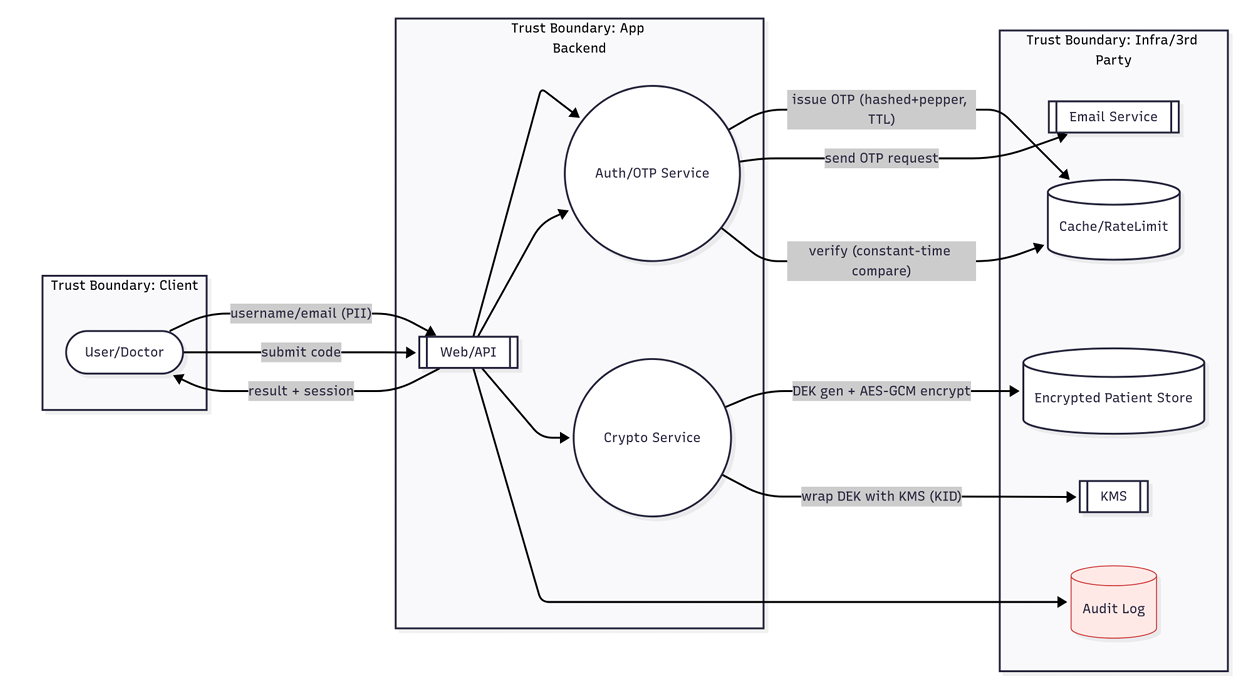
\includegraphics[width=0.9\linewidth]{security_aware_data_flow.png}
  \caption{Security-aware data flow diagram annotating encryption, logging, and boundary controls.}
  \label{fig:security_flow}
\end{figure}

\begin{figure}[t]
  \centering
  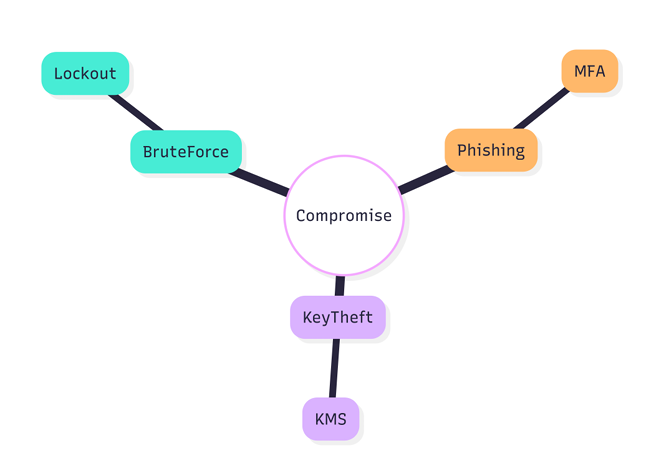
\includegraphics[width=0.85\linewidth]{threat_model_quickview.png}
  \caption{Threat-model quick view aligning STRIDE categories with mitigations across components.}
  \label{fig:threat_model}
\end{figure}

\begin{figure}[t]
  \centering
  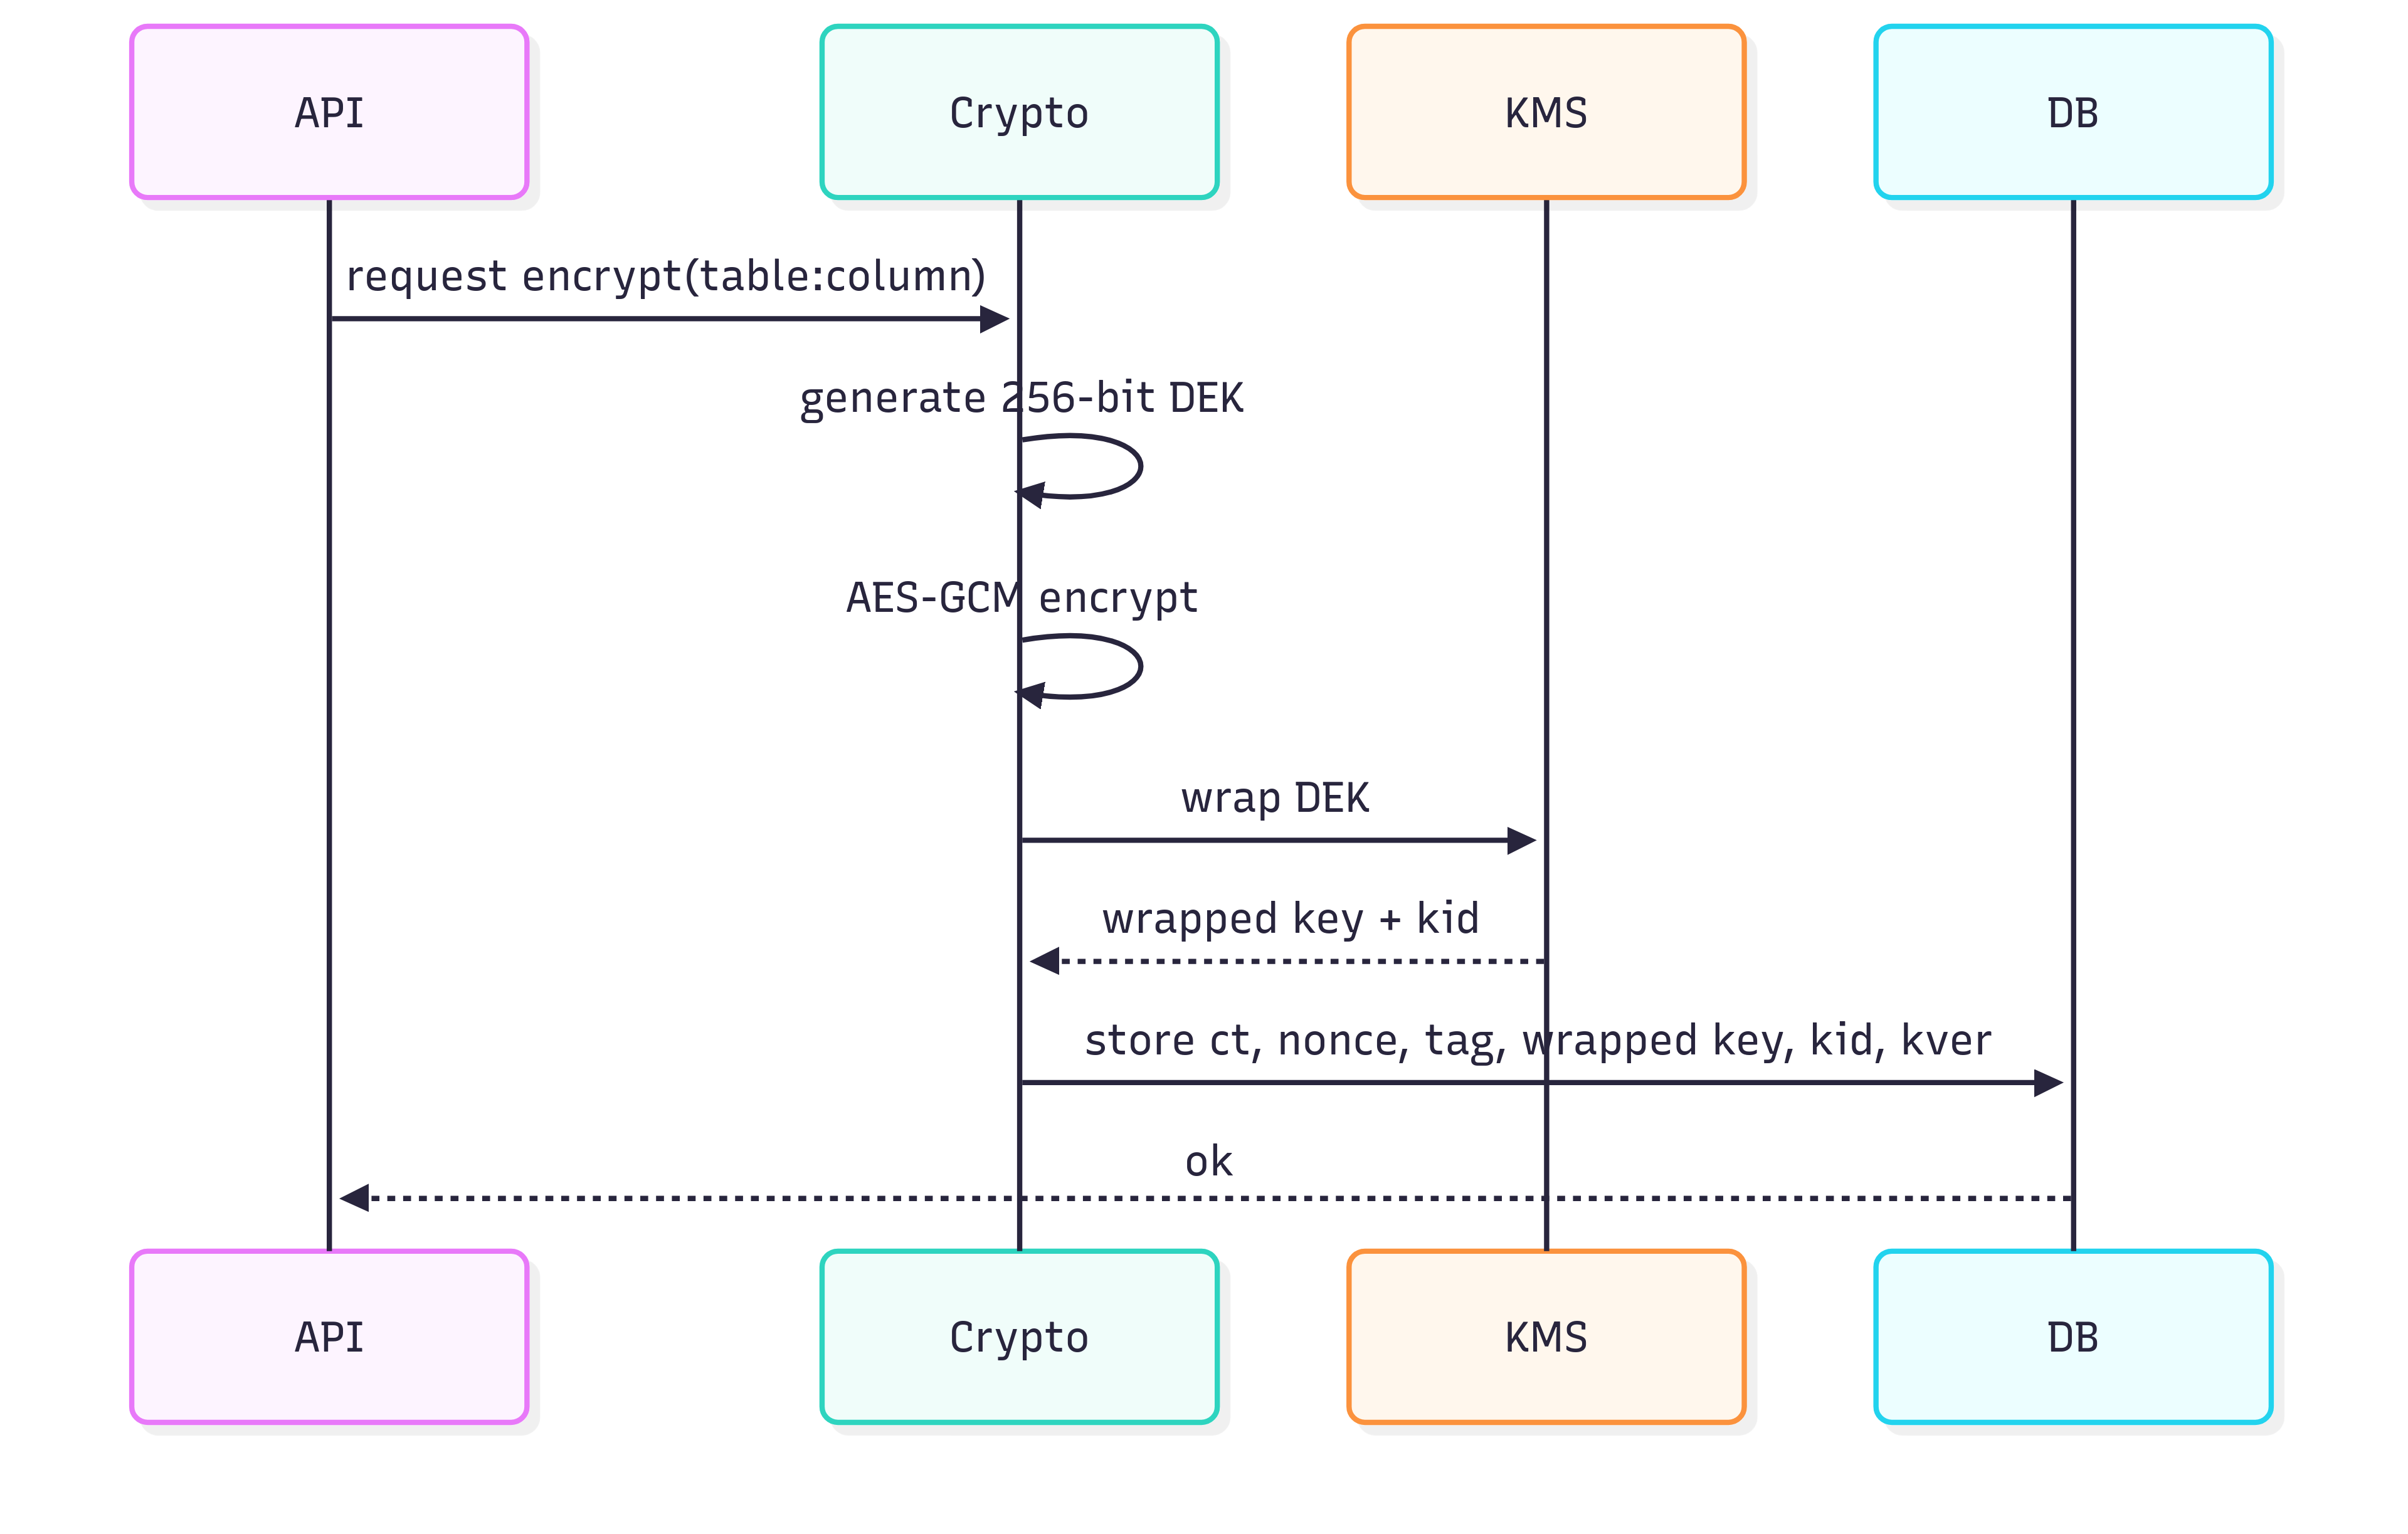
\includegraphics[width=0.9\linewidth]{encryptiondecryption_sequence.png}
  \caption{Sequence diagram for encryption and decryption pathways safeguarding sensitive artifacts.}
  \label{fig:enc_sequence}
\end{figure}

\begin{figure}[t]
  \centering
  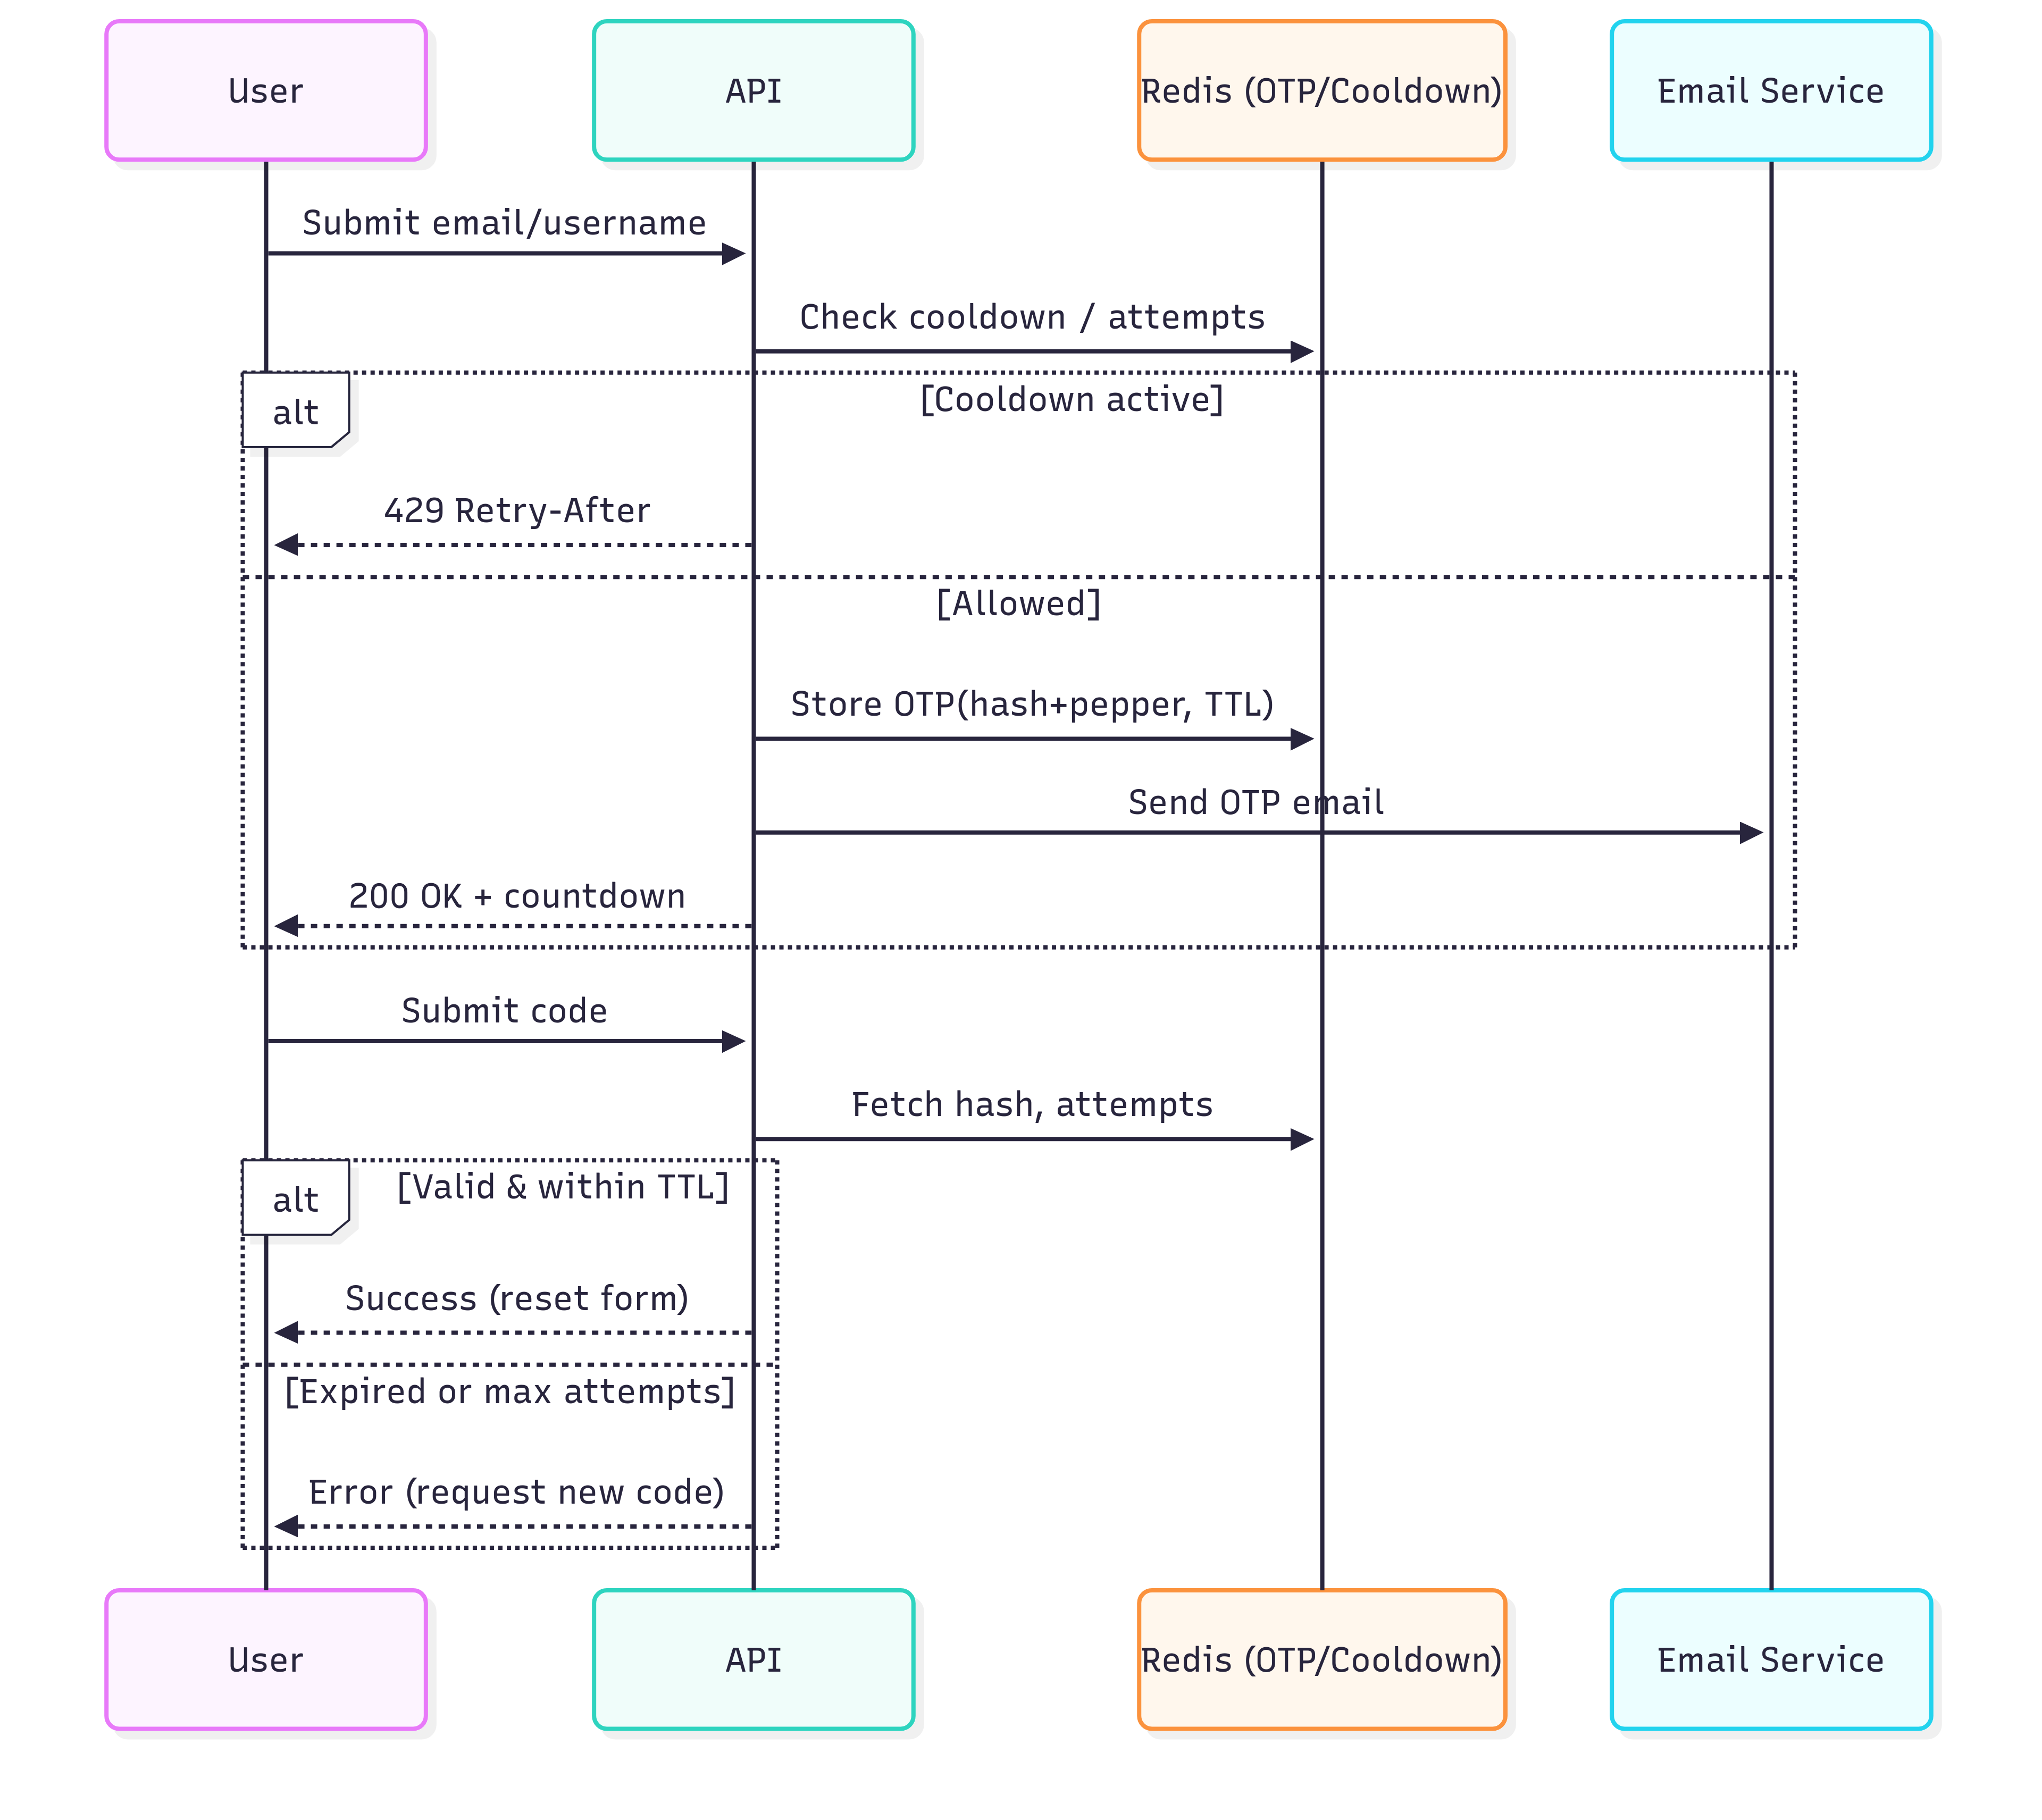
\includegraphics[width=0.9\linewidth]{sequence_of_interactions.png}
  \caption{Service interaction sequence capturing prediction requests, auditing, and notification hooks.}
  \label{fig:sequence_interactions}
\end{figure}

\begin{figure}[t]
  \centering
  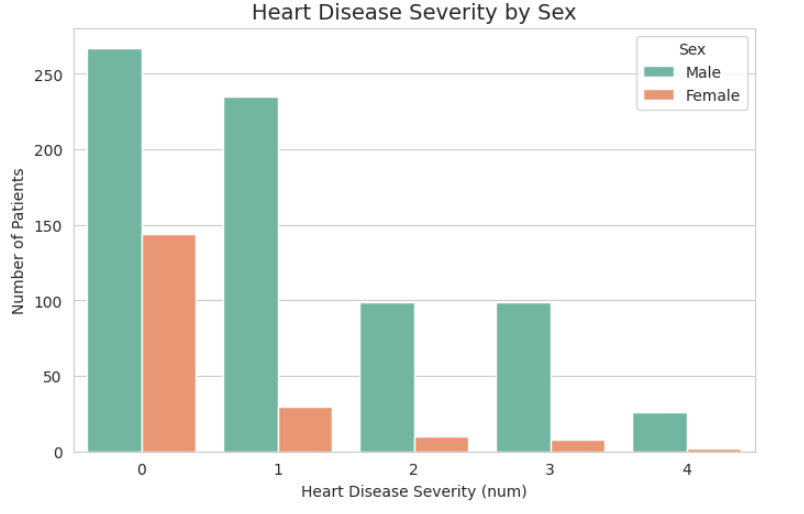
\includegraphics[width=0.9\linewidth]{fig_3_13_should_be_this.png}
  \caption{Defense-in-depth alignment of perimeter, platform, and application safeguards and monitoring loops.}
  \label{fig:defense_layers}
\end{figure}

The application enforces multi-factor authentication during sensitive operations such as password reset. Figure~\ref{fig:bpmn} outlines the two-step verification BPMN flow executed across user, backend, and email service lanes. Complementing this behavioral view, Figure~\ref{fig:dfd} clarifies how OTPs, audit trails, and cooldown tokens traverse storage boundaries with peppered hashing and time-to-live enforcement.

Authentication lifecycle diagrams in Figures~\ref{fig:otp_state} and \ref{fig:pwd_reset_bpmn} expand these processes, while Figure~\ref{fig:sequence_interactions} links OTP issuance, verification, and audit logging across cooperating services.

\begin{figure}[t]
  \centering
  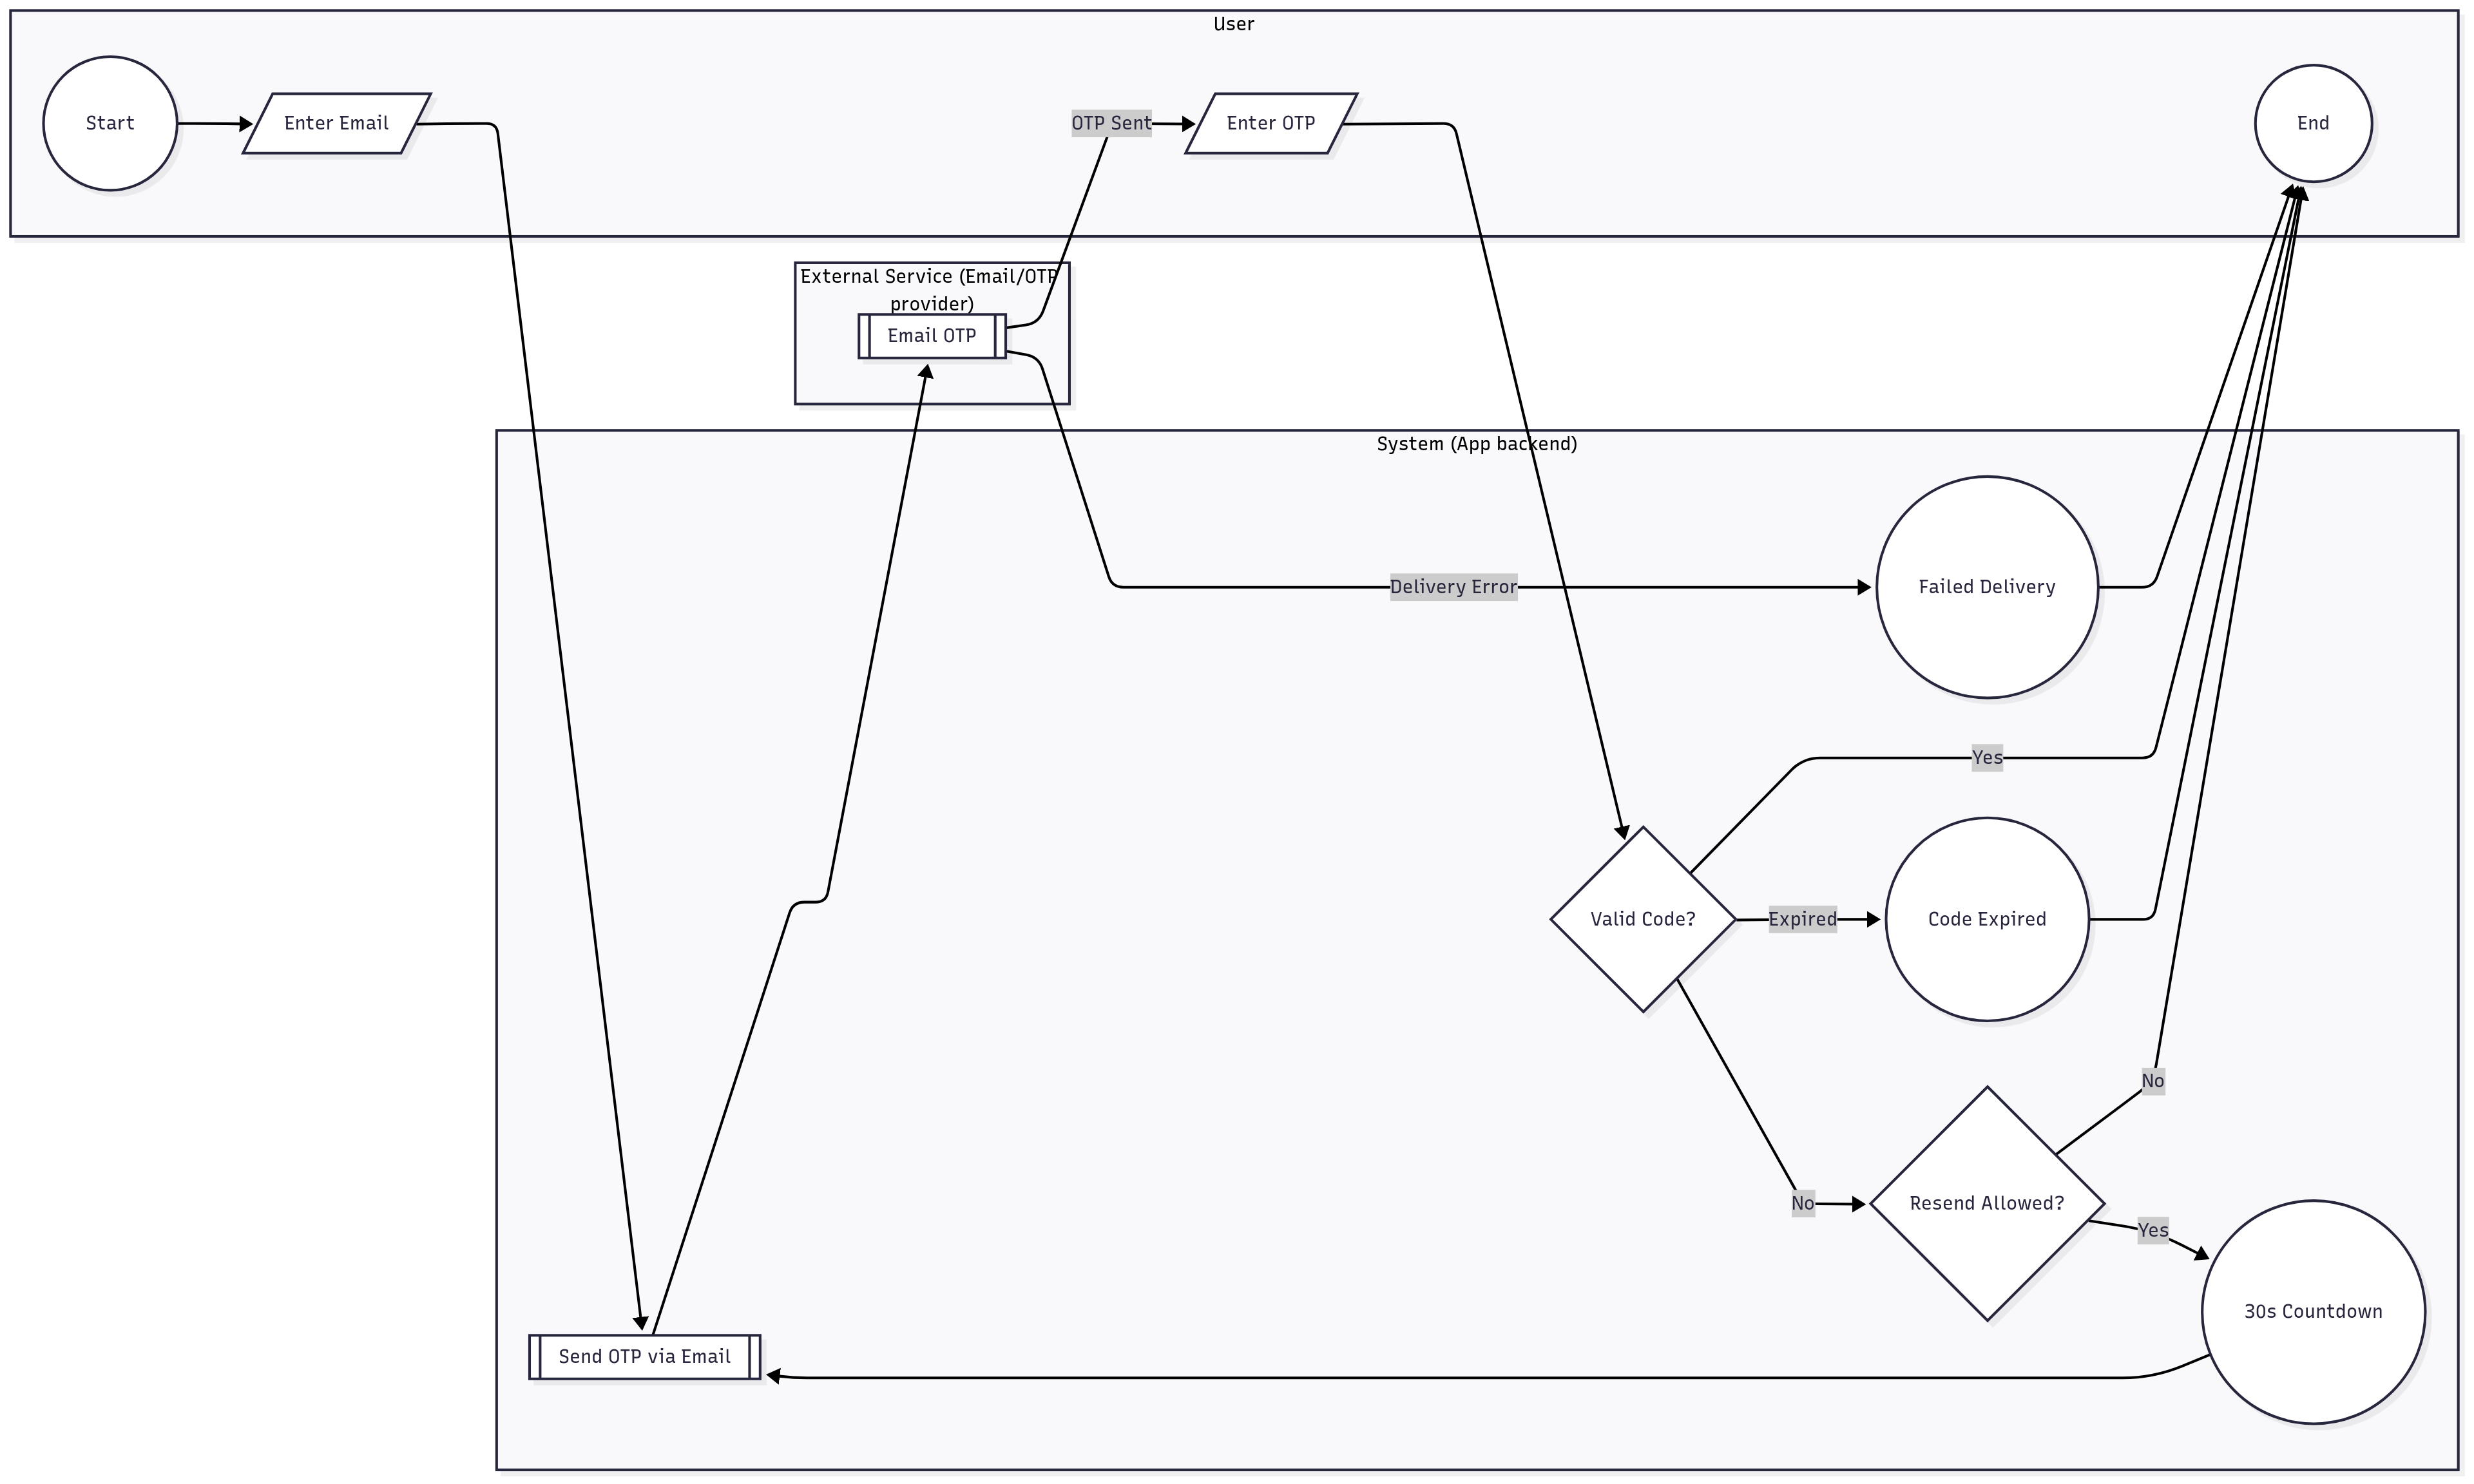
\includegraphics[width=0.9\linewidth]{bpmn_for_two_step_verification.png}
  \caption{BPMN diagram for two-step verification with resend cooldown.}
  \label{fig:bpmn}
\end{figure}

\begin{figure}[t]
  \centering
  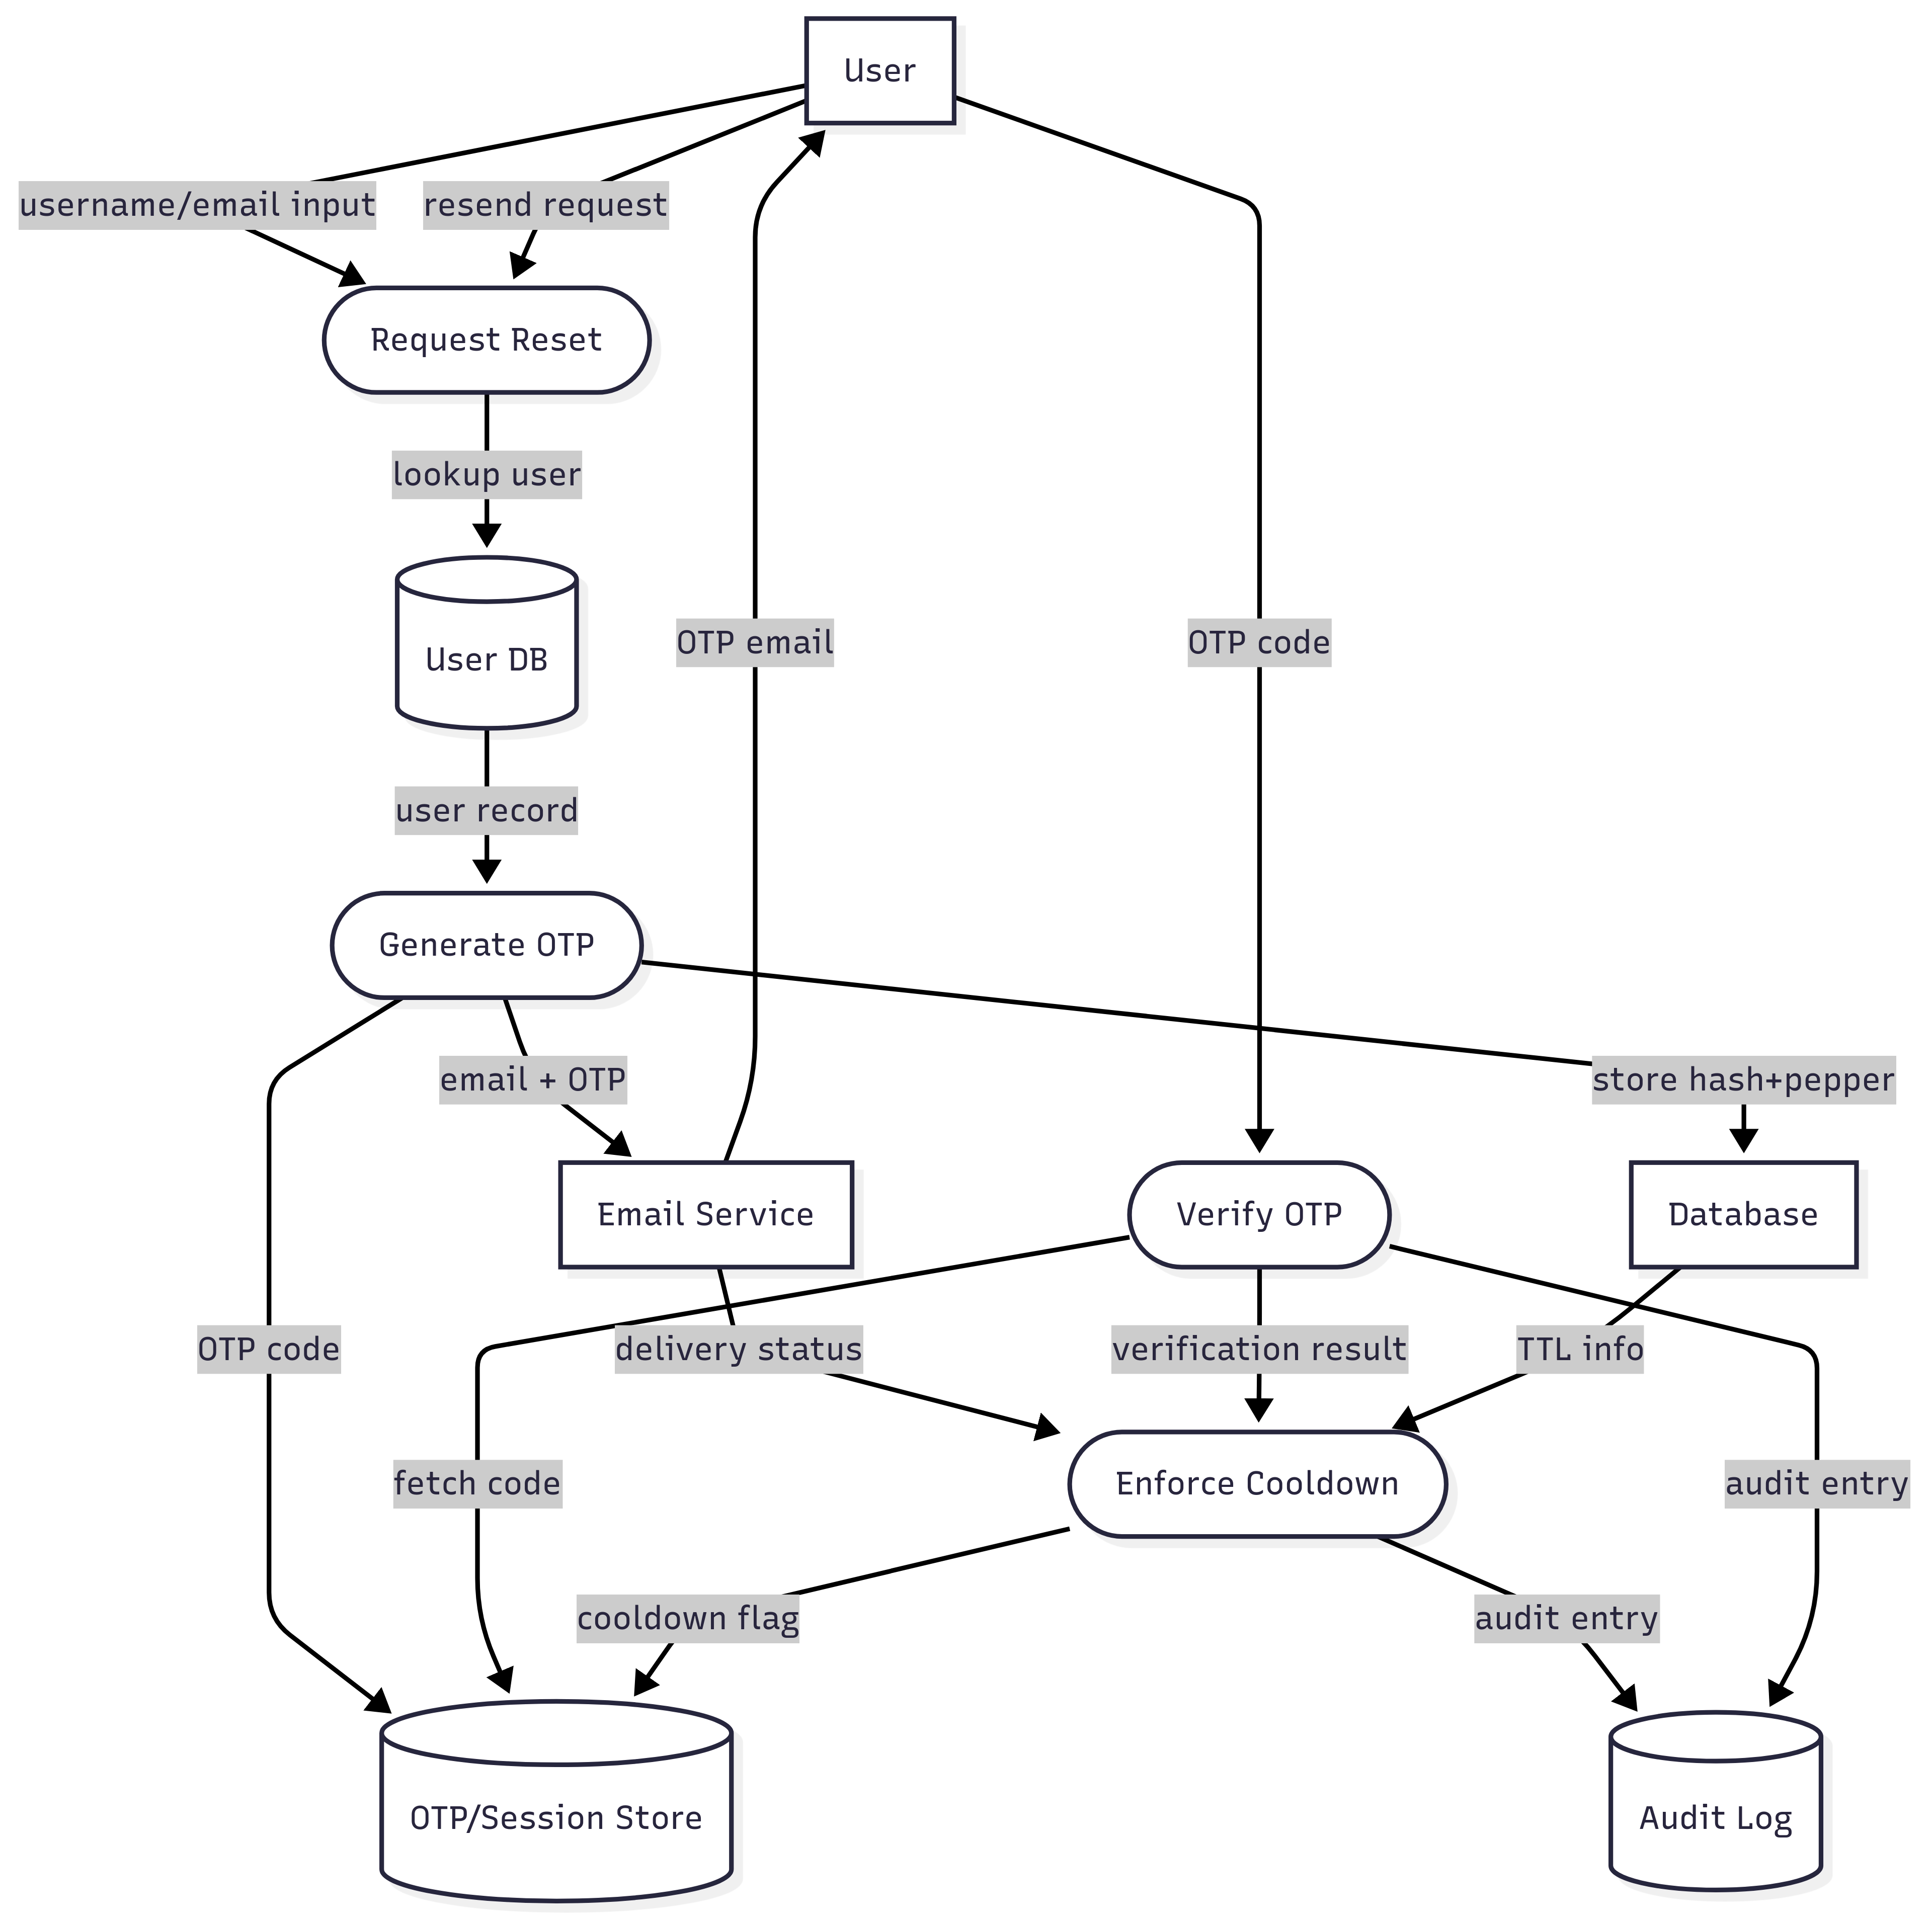
\includegraphics[width=0.9\linewidth]{detailed_data_flow.png}
  \caption{OTP verification data-flow highlighting storage boundaries and audit trails.}
  \label{fig:dfd}
\end{figure}

\begin{figure}[t]
  \centering
  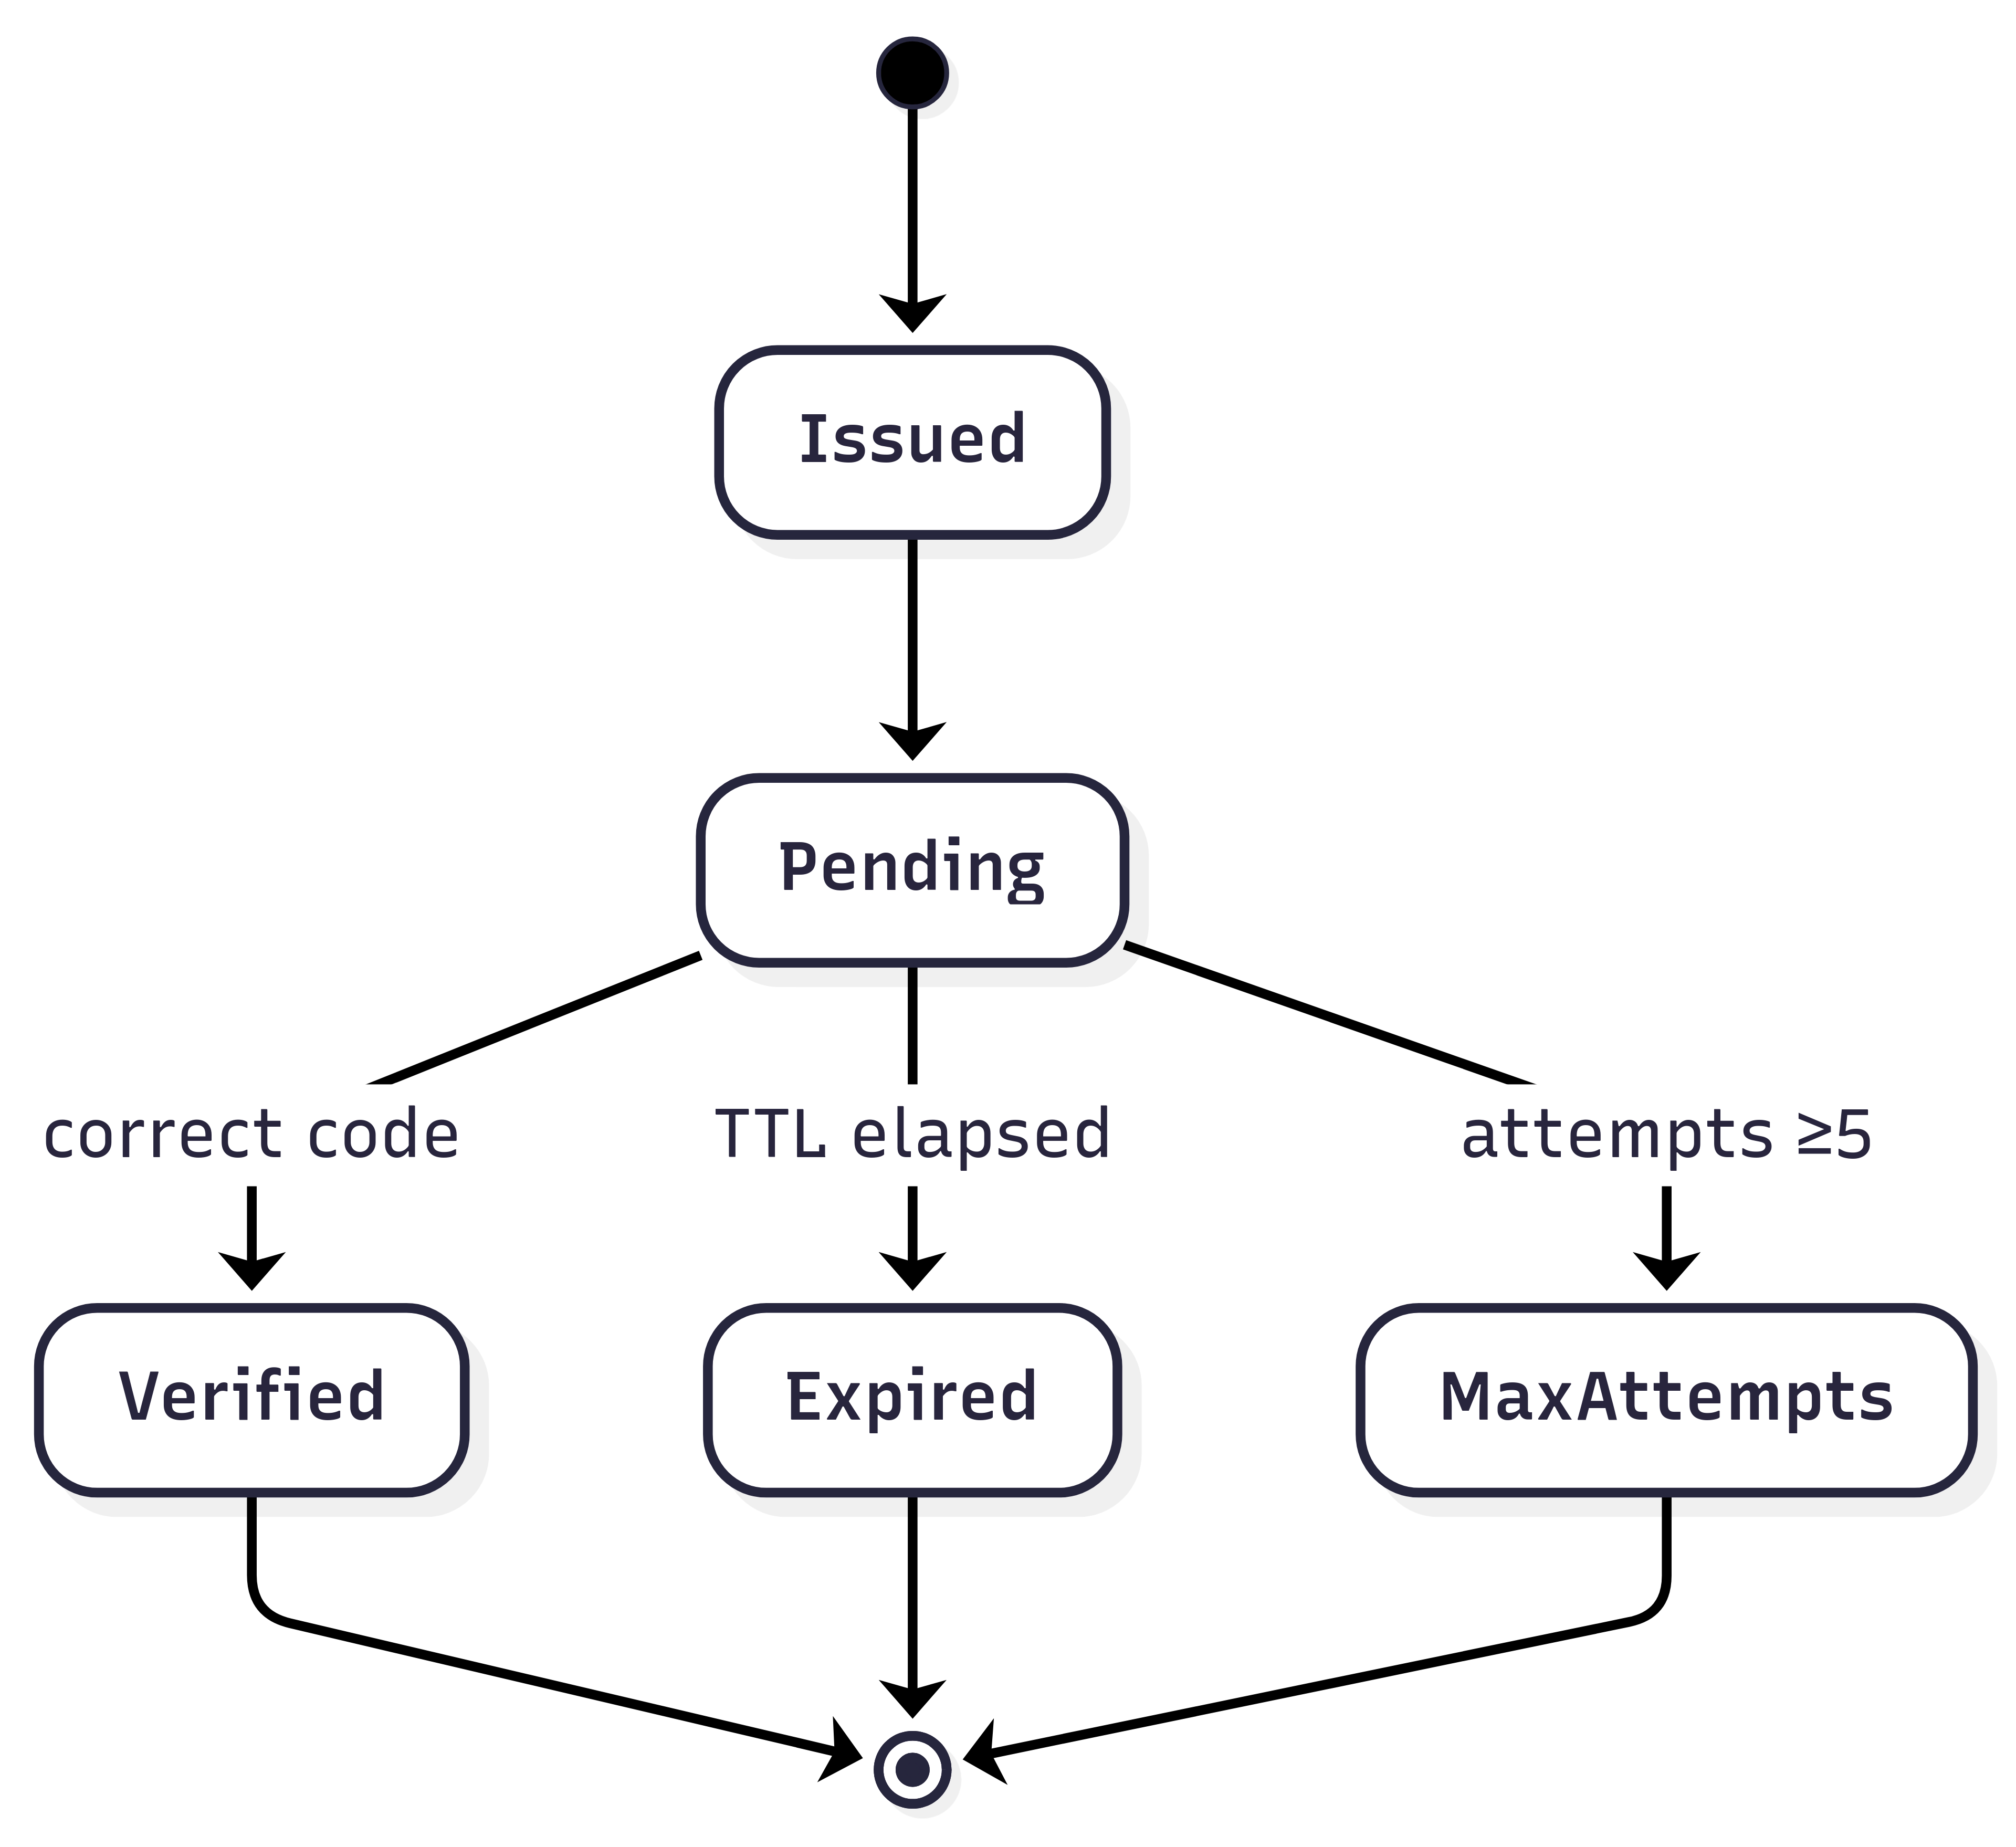
\includegraphics[width=0.85\linewidth]{otp_lifecycle_state_machine.png}
  \caption{OTP lifecycle state machine covering issuance, verification, expiration, and revocation.}
  \label{fig:otp_state}
\end{figure}

\begin{figure}[t]
  \centering
  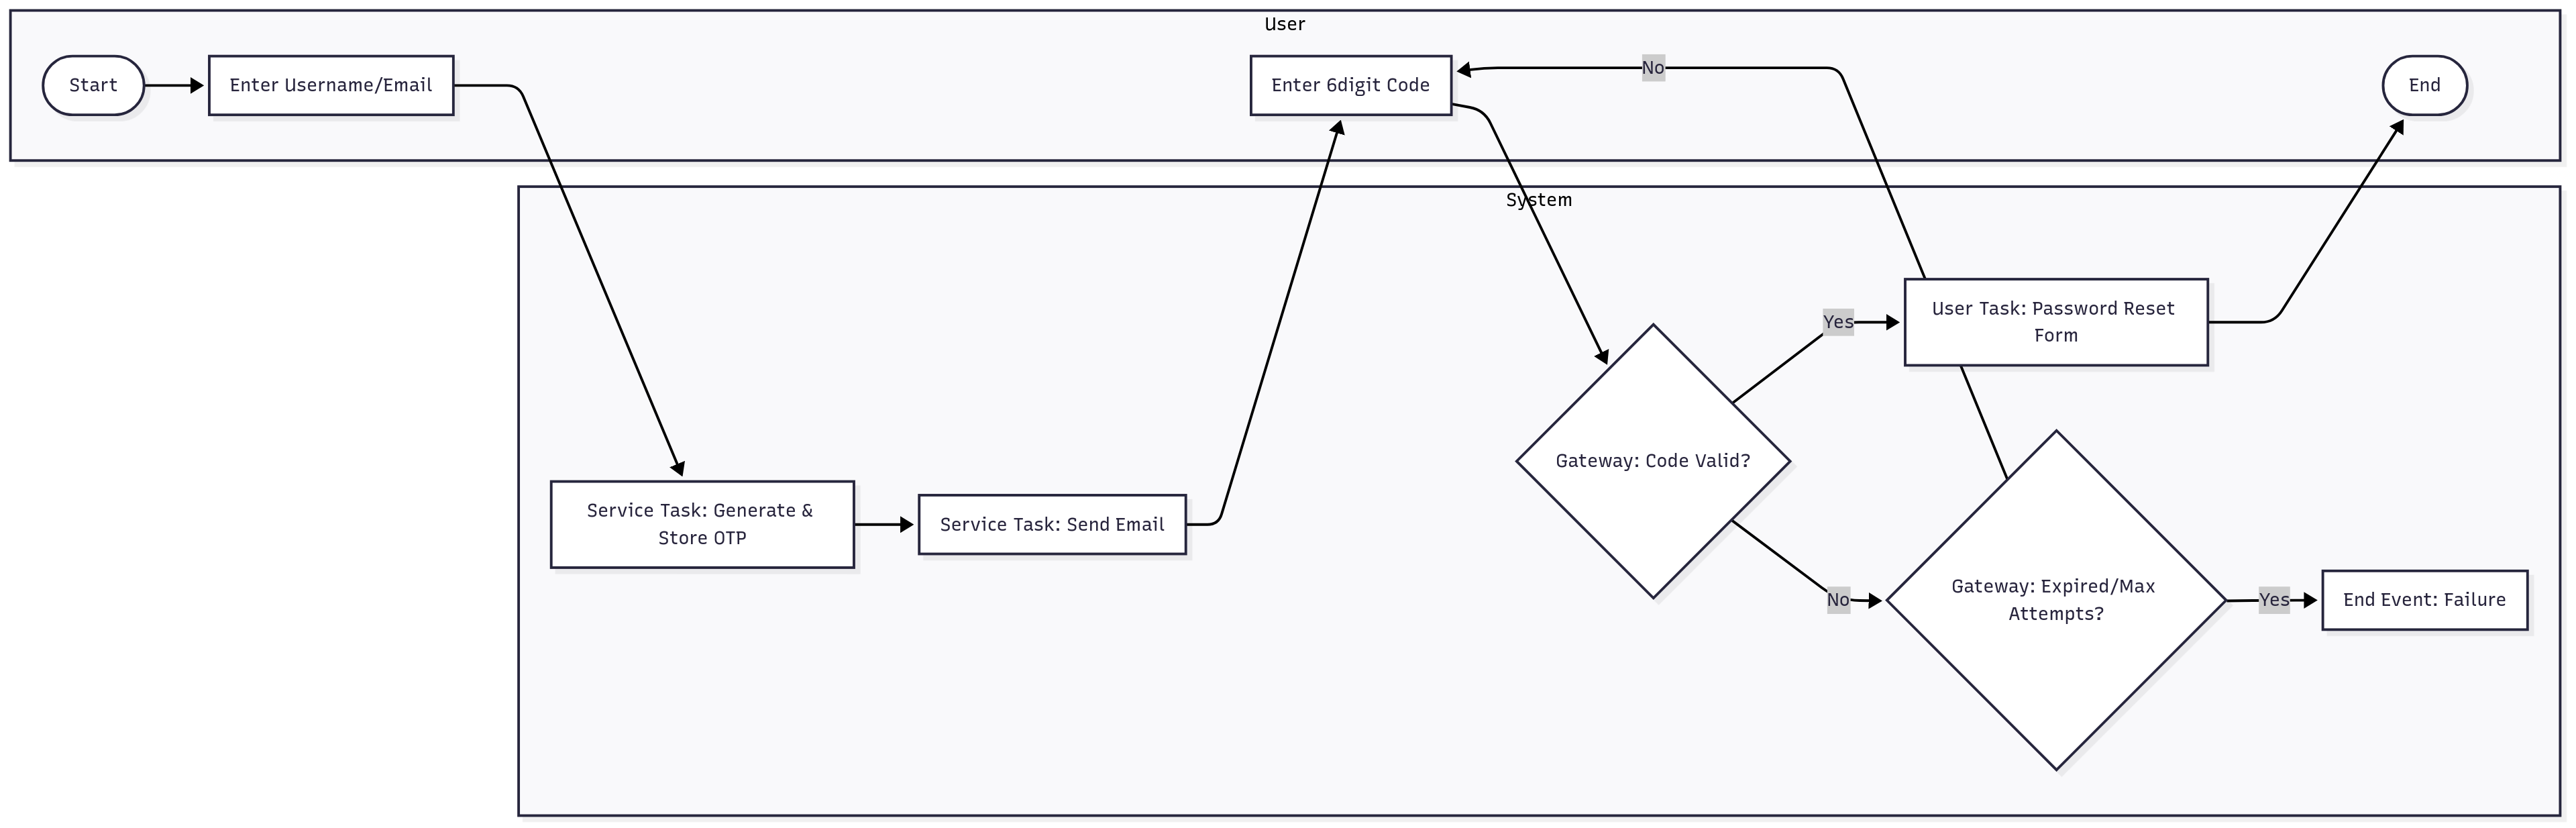
\includegraphics[width=0.85\linewidth]{password_reset_bpmn_process.png}
  \caption{Password reset BPMN process integrating MFA, cooldowns, and audit checkpoints.}
  \label{fig:pwd_reset_bpmn}
\end{figure}

\section{Experimental Evaluation}
\subsection{Machine Learning Performance}
The stratified 70/15/15 data split described in Section~\ref{sec:methods} yielded 644 training, 138 validation, and 138 test encounters. Hyper-parameter tuning maximized validation AUC, after which the best configurations were re-fit on the combined train+validation folds and assessed on the held-out test set. Table~\ref{tab:metrics} summarizes the principal metrics. Both ensembles surpassed 0.91 weighted F1-score; XGBoost delivered marginally higher recall while the Random Forest maintained competitive precision. Receiver-operating characteristic curves exceeded 0.98 AUC for both models, and reliability diagrams confirmed that Platt calibration kept predicted probabilities within 2\% of empirical risk across deciles. Error analysis highlighted borderline patients with normal cholesterol yet atypical angina as the dominant false negatives, whereas false positives typically featured elevated blood pressure but normal thallium scans. Feature-attribution plots reaffirmed clinical priors: \textit{oldpeak}, \textit{cp}, \textit{thal}, \textit{ca}, and \textit{thalach} contributed most strongly across ensembles.

\begin{table}[t]
  \caption{Held-Out Performance Metrics}
  \label{tab:metrics}
  \centering
  \begin{tabular}{lcccc}
    \toprule
    Model & Accuracy & Precision & Recall & F1-score \\
    \midrule
    Random Forest & 0.912 & 0.93 & 0.91 & 0.92 \\
    XGBoost & 0.920 & 0.94 & 0.92 & 0.93 \\
    \bottomrule
  \end{tabular}
\end{table}

\subsection{Testing Strategy}
Automated unit tests (n=142) covered preprocessing, encryption, PDF rendering, and inference utilities with 89\% line coverage. Integration tests executed via Flask's test client validated authentication flows, RBAC decorators, CSV ingestion, asynchronous task completion, and encryption boundaries using an in-memory SQLite instance and stubbed external services. Scenario-based acceptance scripts replicated high-priority user journeys: MFA enrollment and recovery, doctor-only dashboards, SuperAdmin approvals, batch uploads exceeding 500 rows, simulation tooling, and the research viewer. Failures surfaced during development---notably improper cooldown handling for OTP resend---were rectified and locked with regression tests. Continuous integration orchestrated by GitHub Actions runs the full suite on each push, gating releases on green builds.

\subsection{System Performance and Security Evaluation}
Client-observed prediction latency averaged 270~ms (p95: 318~ms) including envelope encryption and template rendering. Batch pipelines processed 500-row CSV uploads in 2.3~s on a four-core staging node, with Celery workers keeping UI threads responsive. Enabling encryption introduced a 9.8~ms median overhead per database transaction, while Argon2id hashing with 256~MiB memory and a parallelism factor of two completed under 120~ms on commodity hardware. MFA verification---password plus TOTP/email code---completed in roughly 820~ms end to end. Fault-injection drills confirmed graceful degradation: simulated KMS outages temporarily blocked PHI reads while leaving non-sensitive modules operational; email delivery delays surfaced progress indicators without leaking code validity windows. Audit trails recorded 100\% of privileged operations in tamper-evident tables, and periodic log-diff checks verified integrity seals.

\section{Discussion}
\subsection{Interpretation of Predictive Findings}
The comparative evaluation shows that both ensembles supply clinically meaningful discrimination with balanced precision and recall. Consistent with prior work, boosting delivered a modest recall advantage, making it attractive for triage workflows where sensitivity dominates \cite{chen2016xgboost}. Nevertheless, Random Forest remained competitive while offering simpler retraining semantics and native feature aggregation \cite{breiman2001random}. Threshold selection therefore remains an operational decision: sites prioritizing high recall may lower alert thresholds and pair models with downstream review queues, whereas resource-constrained clinics may raise thresholds to minimize false positives. Calibrated probability outputs and clinician-facing SHAP summaries help contextualize each prediction, reducing overreliance on raw scores and supporting shared decision making \cite{lundberg2017unified}.

\subsection{Security, Usability, and Deployment Considerations}
Heartlytics demonstrates that security-by-design need not compromise responsiveness or usability. Envelope encryption, Argon2id hashing, MFA, and RBAC added only millisecond-scale overhead yet materially strengthened confidentiality and integrity guarantees \cite{dworkin2007recommendation, biryukov2015argon2, ferraiolo2001proposed}. WCAG-aligned theming, motion sensitivity, and printable reports address clinician usability concerns identified in the thesis literature review \cite{w3c_wcag21, oshero2012improving}. Asynchronous workers and audit logging further bridge the gap between academic prototypes and production expectations by ensuring observability, resilience, and traceability \cite{howard2006security, celery}.

\subsection{Limitations}
Two limitations mirror those acknowledged in the dissertation. First, external validity is constrained by the size and demographics of the UCI cohorts; future deployments should recalibrate on contemporary, site-specific data and monitor drift over time \cite{mitchell2019model}. Second, fairness analysis was limited to coarse demographic slices (sex); more granular subgroup audits with confidence intervals are needed before high-stakes adoption \cite{barocas2019fairness}. Probability calibration and threshold policies likewise require continual review to stay aligned with local prevalence and capacity \cite{platt1999probabilistic}. Finally, while the system enforces strong security primitives, formal penetration testing and blue-team exercises remain outstanding.

\section{Conclusion and Future Work}
This work distilled the thesis contributions into an IEEE manuscript, evidencing that machine-learning-driven screening can coexist with rigorous security, testing, and usability practices. The resulting platform couples calibrated ensembles with envelope encryption, MFA, and RBAC, all validated through automated and scenario-based testing. Future research will extend along four axes: (i) federated or privacy-preserving learning to accommodate multi-institutional datasets without centralizing PHI; (ii) continuous calibration, drift, and fairness monitoring with automated alerts; (iii) richer feature spaces integrating medications, longitudinal vitals, and FHIR-based interoperability; and (iv) operational hardening that encompasses penetration tests, chaos drills for key-management and email dependencies, and comprehensive model documentation.
\FloatBarrier

\begin{thebibliography}{00}
\bibitem{janosi1988uci} A.~Janosi, W.~Steinbrunn, M.~Pfisterer, and R.~Detrano, ``Heart disease dataset,'' UCI Machine Learning Repository, 1988.
\bibitem{breiman2001random} L.~Breiman, ``Random forests,'' \emph{Machine Learning}, vol.~45, no.~1, pp.~5--32, 2001.
\bibitem{chen2016xgboost} T.~Chen and C.~Guestrin, ``XGBoost: A scalable tree boosting system,'' in \emph{Proceedings of the 22nd ACM SIGKDD International Conference on Knowledge Discovery and Data Mining}, 2016, pp.~785--794.
\bibitem{zhang2021heart} D.~Zhang, Y.~Yang, and X.~Y. Chen, ``Heart disease prediction based on the embedded feature selection method and deep neural network,'' \emph{Journal of Healthcare Engineering}, vol.~2021, pp.~1--10, 2021.
\bibitem{pedregosa2011scikit} F.~Pedregosa \emph{et~al.}, ``Scikit-learn: Machine learning in Python,'' \emph{Journal of Machine Learning Research}, vol.~12, pp.~2825--2830, 2011.
\bibitem{chawla2002smote} N.~V. Chawla, K.~W. Bowyer, L.~O. Hall, and W.~P. Kegelmeyer, ``SMOTE: Synthetic minority over-sampling technique,'' \emph{Journal of Artificial Intelligence Research}, vol.~16, pp.~321--357, 2002.
\bibitem{platt1999probabilistic} J.~Platt, ``Probabilistic outputs for SVMs and comparisons to regularized likelihood methods,'' in \emph{Advances in Large Margin Classifiers}. MIT Press, 1999, pp.~61--74.
\bibitem{kohavi1995study} R.~Kohavi, ``A study of cross-validation and bootstrap for accuracy estimation and model selection,'' in \emph{Proceedings of the 14th International Joint Conference on Artificial Intelligence}, 1995, pp.~1137--1143.
\bibitem{lundberg2017unified} S.~M. Lundberg and S.-I. Lee, ``A unified approach to interpreting model predictions,'' in \emph{Proceedings of the 31st Conference on Neural Information Processing Systems}, 2017, pp.~4765--4774.
\bibitem{dworkin2007recommendation} M.~Dworkin, ``Recommendation for block cipher modes of operation: Galois/Counter Mode (GCM) and GMAC,'' NIST Special Publication 800-38D, 2007.
\bibitem{googlekms} Google Cloud, ``Envelope encryption with Cloud KMS,'' 2024. [Online]. Available: \url{https://cloud.google.com/kms/docs/envelope-encryption}
\bibitem{awskms} Amazon Web Services, ``Envelope encryption,'' 2024. [Online]. Available: \url{https://docs.aws.amazon.com/kms/latest/developerguide/concepts.html#enveloping}
\bibitem{biryukov2015argon2} A.~Biryukov, D.~Dinu, and D.~Khovratovich, ``Argon2: The memory-hard function for password hashing and other applications,'' in \emph{Proceedings of the IEEE European Symposium on Security and Privacy}, 2016, pp.~292--302.
\bibitem{provos1999bcrypt} N.~Provos and D.~Mazieres, ``A future-adaptable password scheme,'' in \emph{Proceedings of the USENIX Annual Technical Conference}, 1999, pp.~81--92.
\bibitem{grassi2017digital} P.~A. Grassi, M.~E. Garcia, and J.~L. Fenton, ``Digital identity guidelines: Authentication and lifecycle management,'' NIST Special Publication 800-63B, 2017.
\bibitem{mraihi2011totp} D.~M'Raihi, S.~Machani, M.~Pei, and J.~Rydell, ``TOTP: Time-based one-time password algorithm,'' RFC 6238, 2011.
\bibitem{owasp2021} OWASP Foundation, ``OWASP Top 10: Identification and authentication failures,'' 2021. [Online]. Available: \url{https://owasp.org/Top10/}
\bibitem{ferraiolo2001proposed} D.~F. Ferraiolo, R.~Sandhu, S.~L. Gavrila, D.~R. Kuhn, and R.~Chandramouli, ``Proposed NIST standard for role-based access control,'' \emph{ACM Transactions on Information and System Security}, vol.~4, no.~3, pp.~224--274, 2001.
\bibitem{howard2006security} M.~Howard and S.~Lipner, \emph{The Security Development Lifecycle}. Redmond, WA, USA: Microsoft Press, 2006.
\bibitem{shostack2014threat} A.~Shostack, \emph{Threat Modeling: Designing for Security}. Indianapolis, IN, USA: Wiley, 2014.
\bibitem{grinberg2018flask} M.~Grinberg, \emph{Flask Web Development}, 2nd~ed. Boston, MA, USA: O'Reilly Media, 2018.
\bibitem{celery} Celery Project, ``Celery distributed task queue,'' 2024. [Online]. Available: \url{https://docs.celeryq.dev/}
\bibitem{bootstrap5} Bootstrap Authors, ``Bootstrap 5 documentation,'' 2024. [Online]. Available: \url{https://getbootstrap.com/}
\bibitem{reportlab} ReportLab, ``ReportLab user guide,'' 2024. [Online]. Available: \url{https://www.reportlab.com/docs/reportlab-userguide.pdf}
\bibitem{w3c_wcag21} World Wide Web Consortium, ``Web content accessibility guidelines (WCAG) 2.1,'' 2018. [Online]. Available: \url{https://www.w3.org/TR/WCAG21/}
\bibitem{oshero2012improving} J.~A. Osheroff, J.~M. Teich, D.~F. Sittig, B.~S. Sirajuddin, and R.~A. Velasco, \emph{Improving Outcomes with Clinical Decision Support: An Implementer's Guide}, 2nd~ed. Chicago, IL, USA: HIMSS, 2012.
\bibitem{mitchell2019model} M.~Mitchell \emph{et~al.}, ``Model cards for model reporting,'' in \emph{Proceedings of the Conference on Fairness, Accountability, and Transparency}, 2019, pp.~220--229.
\bibitem{barocas2019fairness} S.~Barocas, M.~Hardt, and A.~Narayanan, \emph{Fairness and Machine Learning}. Cambridge, MA, USA: MIT Press, 2019.
\end{thebibliography}

\end{document}
